\documentclass[Japanese]{dicomopapers}
%\documentclass[Japanese,noauthor]{dicomopapers}
\usepackage[dvipdfmx]{graphicx}
\usepackage{latexsym}
\usepackage{url}
\renewcommand{\baselinestretch}{1.0}

\def\Underline{\setbox0\hbox\bgroup\let\\\endUnderline}
\def\endUnderline{\vphantom{y}\egroup\smash{\underline{\box0}}\\}
\def\|{\verb|}



\begin{document}

% 和文表題
\title{BLEビーコンを用いた物体状態推定手法}
% 英文表題
\etitle{Proposal of Object State Estimation Method \\ using BLE Beacon}

% 所属ラベルの定義
\affiliate{1}{愛知工業大学 情報科学部情報科学科}

\author{大鐘 勇輝}{YUKI OGANE}{1}
\author{水野 涼雅}{RYOGA MIZUNO}{1}
\author{梶 克彦}{KATSUHIKO KAJI}{1}




\begin{abstract}
近年IoTの普及によって様々なセンサが家電に取り付けられ, そこから得られる情報によりライフログデータの取得が可能となった.
ライフログデータはセンサが搭載されている家電では収集が容易であるが, 特殊なセンサの無い家電や扉, 椅子といった家具ではデータの収集が難しい.
これまでそのような家電や家具などの状態推定には加速度センサやWi-Fiの電波が用いられてきたが, 移動の有無や推定対象物の大きさによって推定精度が大きく左右される問題があった.
そこで本研究では, Bluetooth Low Energyビーコン(以下BLEビーコンと呼称)を家電や家具などモノの中に直接入れ, 状態によって変化するBLEビーコンの電波強度をもとに推定を行う手法を提案する.
BLEビーコンの電波は微弱であるため, 環境の変化による電波の乱れが発生しやすい.
そのため提案手法では, 取得した電波強度データに対しデジタルフィルタの一つであるローパスフィルタを適用しノイズの除去を行う.
また, 本手法では推定対象物の移動も考慮するため, 簡単な閾値処理だけでは推定が困難である.
そこで, 安定センシング区間という概念を導入し, 電波強度が安定している区間を見つけ状態を判断する閾値を動的に変えることによって推定精度の向上を試みた.
安定センシング区間の判定には, 吉澤ら\cite{ips-chube}が研究内で使用しているεチューブを利用している.
上記の方法を三種類のモノに適用し推定精度を確かめた.
その結果, いずれも高い精度で状態推定できることを実証した.

\textgt{\\キーワード} : ビーコン電波による物体の状態推定, 安定センシング区間, εチューブ, ライフログ


\end{abstract}

% 表題などの出力
\maketitle

% 本文はここから始まる
\section{はじめに}
通信インフラの整備とIoTの発展により, 現在では様々なモノがインターネットに繋がるようになった.
エアコンや照明, 家の鍵から車に至るまで, 数年前ではインターネットとは無関係だったものが今では当たり前のようにインターネットに接続されている.
IoTに対応した家電は遠隔からの機器の操作や 機器の状態の通知, 使用ログの保存といったことが可能であり, 例えばIoTに対応したエアコンでは家の外から電源のON・OFFや電気使用量のログの確認ができる.
そうした利便性から日々新たなIoT家電が生み出され続けており, 総務省が公開している資料\cite{soumusyo}によると2020年には約300億のIoTデバイスが稼働していると予想されている.
IoTデバイスの増加により家中にそれらが設置されると, そこから得られる使用データから行動パターンといったライフログのデータが取得できる.
ライフログのデータは, 環境に合わせた電力制御や老人の異常行動の検知など幅広い分野への応用が期待できる.

しかし, これらのデータはIoTに対応した家電でないと取得できず, 金庫や椅子, 扉といった家電以外のモノではセンサが無いためデータ収集が不可能という問題がある.
この解決策として, (1)加速度センサや回転センサを使う方法と, (2)Wi-Fi電波のチャネルの状態情報を使った方法がある.
(1)の方法は直接モノの動きを観測できるため安定した精度で状態推定ができる反面, センサー単体での動作が難しく取得したデータの保存・解析に専用の機器が必要である. %消費電力が大きく定期的に電池の交換が必要であるでも良いかも
また(2)の方法では対象物のそれぞれにセンサを付ける必要が無い一方, 状態の推定にWi-Fi電波の反射波を用いるという特徴から小さな対象物への適用は不得意である.

そこで本研究では汎用的な機器のみで動作でき, かつ小さな対象物でも高い精度で状態推定できる手法を提案する.
具体的には日常の生活空間内における家電・家具の内部にBluetooth Low Energyビーコン(以下BLEビーコン)を設置し, 送信される電波をスマートフォンで受信した際の受信電波強度をもとにモノの状態推定を行う手法である.
BLEビーコンは小型・省電力なため長期間の稼働が可能であり, また電波が微弱なので障害物の有無により電波強度が変化しやすく状態推定に適している.
加えてBLEビーコンの電波はスマートフォンで受信できるため, 電波の受信に特別な機器を必要とせず, UUID, major, minorの情報から各BLEビーコンを識別することができるため, 1台のスマートフォンで複数のBLEビーコンを監視することができる.

システム概要図を図\ref{abst}に示す.
本手法では, BLEビーコンを金庫や冷蔵庫であれば開閉を行う蓋や扉の部分に, 椅子では座面のクッション下へ設置し推定を行う.
この時, 受信したデータをそのまま使用するとノイズの影響で正確に推定を行うことができない.
そのため, ノイズを取り除くため受信したデータに対してフィルタ処理を施し, 状態の推定を行う.

本稿の構成は以下の通りである.
2章では, 屋内日常物における状態推定に関する既存研究を紹介し, その問題点を述べる.
3章では, 既存手法における問題点を解決するために, 本研究のBLEビーコンを使用してモノの状態推定行う手法を述べる.
4章では, 本研究で提案した手法の評価と考察を行う.
最後に5章で, 本研究のまとめと考察を行う.


%ーーーーーーーーーーーーーーーーーーーーーーーーーーーーーーーーーーーーーーーーーーーーーーーーー
%ーーーーーーーーーーーーーーーーーーーーーーーーーーーーーーーーーーーーーーーーーーーーーーーーー

% 図の挿入
\begin{figure}[ht]
 \centering
 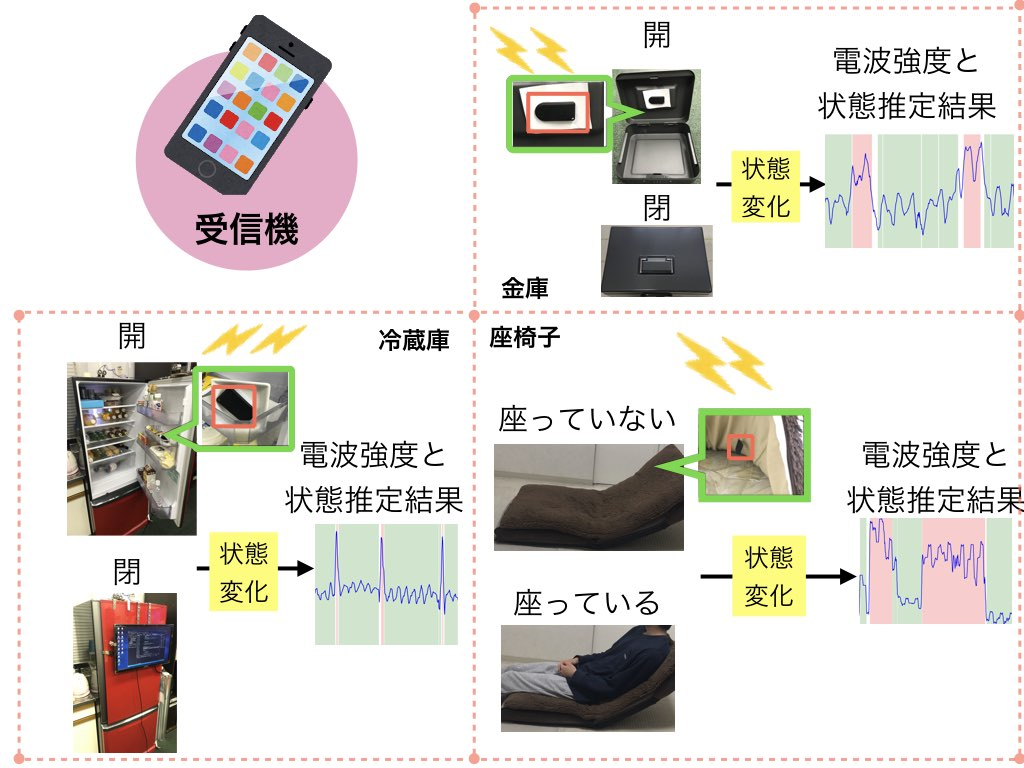
\includegraphics[width=8.5cm]{abst.jpeg}
 \caption{システム概要図}
 \label{abst}
\end{figure}

\section{関連研究}
室内にある物の状態推定には, 加速度センサや振動センサなどを利用する方法やWi-Fiの電波を利用する方法など様々な手法が提案されてきた.
前川ら\cite{TagAndThink}は様々なセンサを搭載したセンサノードをモノに取り付け, そこから得られるセンサ情報と事前に用意しておいたそのモノ固有の状態遷移図を比較することにより, 自動でモノの状態と何に付けられているのか推定をしている.
角速度や照度などから, センサノードが取り付けられている状況や状態変化を検出するという手法である.
この手法ではセンサノードがどんなモノに付いていてどんな状態変化をしたかを推定することが可能である.


消費電力の変化から電気機器の状態推定を行っている研究がいくつかある.
上田ら\cite{sairyu}は機器やコンセントごとの消費電力を計測できる細粒度電力センサを使用し, 電気機器の電力消費の変化から浪費電力の検出・分類を行っている.
また, 山田ら\cite{energy}は電気機器の運転モードの切り替えや開閉などの状態変化によって起こる消費電力の変化から状態の推定を行い, 複数の電気機器の状態変化を時系列に並べることで人物の位置推定を行っている.
これら二つの手法では, 電気機器の状態変化から起こる消費電力の増減に着目し推定を行っているため, 電化製品に対しては有効な手法ある.
一方で, 電気を用いない家具や雑貨に対しては適用することが不可能である.


日常生活空間内での扉の開閉推定を行う尾原ら\cite{WifiChannel}の研究では, Wi-Fiのチャンネル状態情報を用いて物体の移動から発生するドップラー効果や電波の到来方向からドアの開閉状態を検知している.
この研究では推定の対象物は扉でありある程度大きさがあるモノであるため, Wi-Fiチャネル状態情報に影響を及ぼしやすくこの手法は有効である.

しかし, 小さな箱の開閉や移動した先での状態変化を推定する事は難しいため, 我々はBLEビーコンを用いて電波強度の変化から状態変化の推定を行うことにした.
BluetoothLowEnergyの技術は近年, 広告配信や位置推定など様々な用途に使われている.
例えばSNSサービスを提供しているLINEでは, BLEビーコンを使用して決済ができるサービスを提供している.\cite{bleUse}



BLEビーコンの受信機との距離による減衰や, 障害物による電波の減衰などによって変化する電波強度をもとに, 複数の受信機を用いて位置の推定や状態の推定をする研究が数多く行われている\cite{IoMT}, \cite{tandem}, \cite{blespot}, \cite{LANgate}, \cite{en-door}.
これらで利用されているように, BLEビーコンの電波は微弱であるため数mの距離の変化や障害物などにより電波の減衰が起こる.
この現象を利用し我々は日常の生活空間内におけるモノの状態変化推定を行う.





%ーーーーーーーーーーーーーーーーーーーーーーーーーーーーーーーーーーーーーーーーーーーーーーーーー
%ーーーーーーーーーーーーーーーーーーーーーーーーーーーーーーーーーーーーーーーーーーーーーーーーー





\section{物体内部に配置したBLEビーコンの電波強度を用いた状態推定}
本研究では冷蔵庫や金庫, 座椅子などの内部に図\ref{beacon}のBLEビーコンを設置し, その電波強度の変化からモノの状態推定を行う.
冷蔵庫(図\ref{freezer})では扉の棚部分, 金庫(図\ref{safe})では開閉する蓋の部分, 座椅子(図\ref{chair})では人が座る座面の部分や背もたれの部分のカバー裏へBLEビーコンの設置を行う.
これにより扉の開閉や人の着座などのモノの状態変化からBLEビーコンの遮蔽状態が変化するため, 外側に設置する受信機からみたBLEビーコンの電波強度が変化する.
この変化する電波強度をもとに設置対象の状態変化の推定を行う.


% 図の挿入
\begin{figure}[ht]
    \centering
    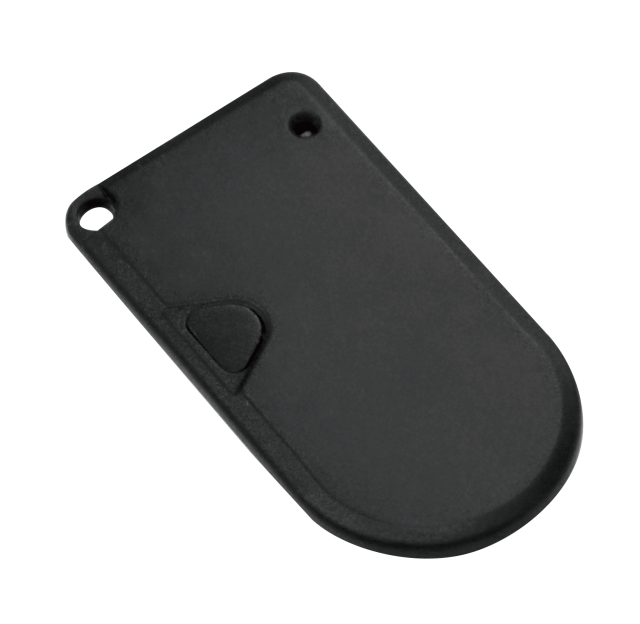
\includegraphics[width=3cm]{ble.png}
    \caption{BLEビーコン}
    \label{beacon}
   \end{figure}
\begin{figure}[ht]
    \centering
    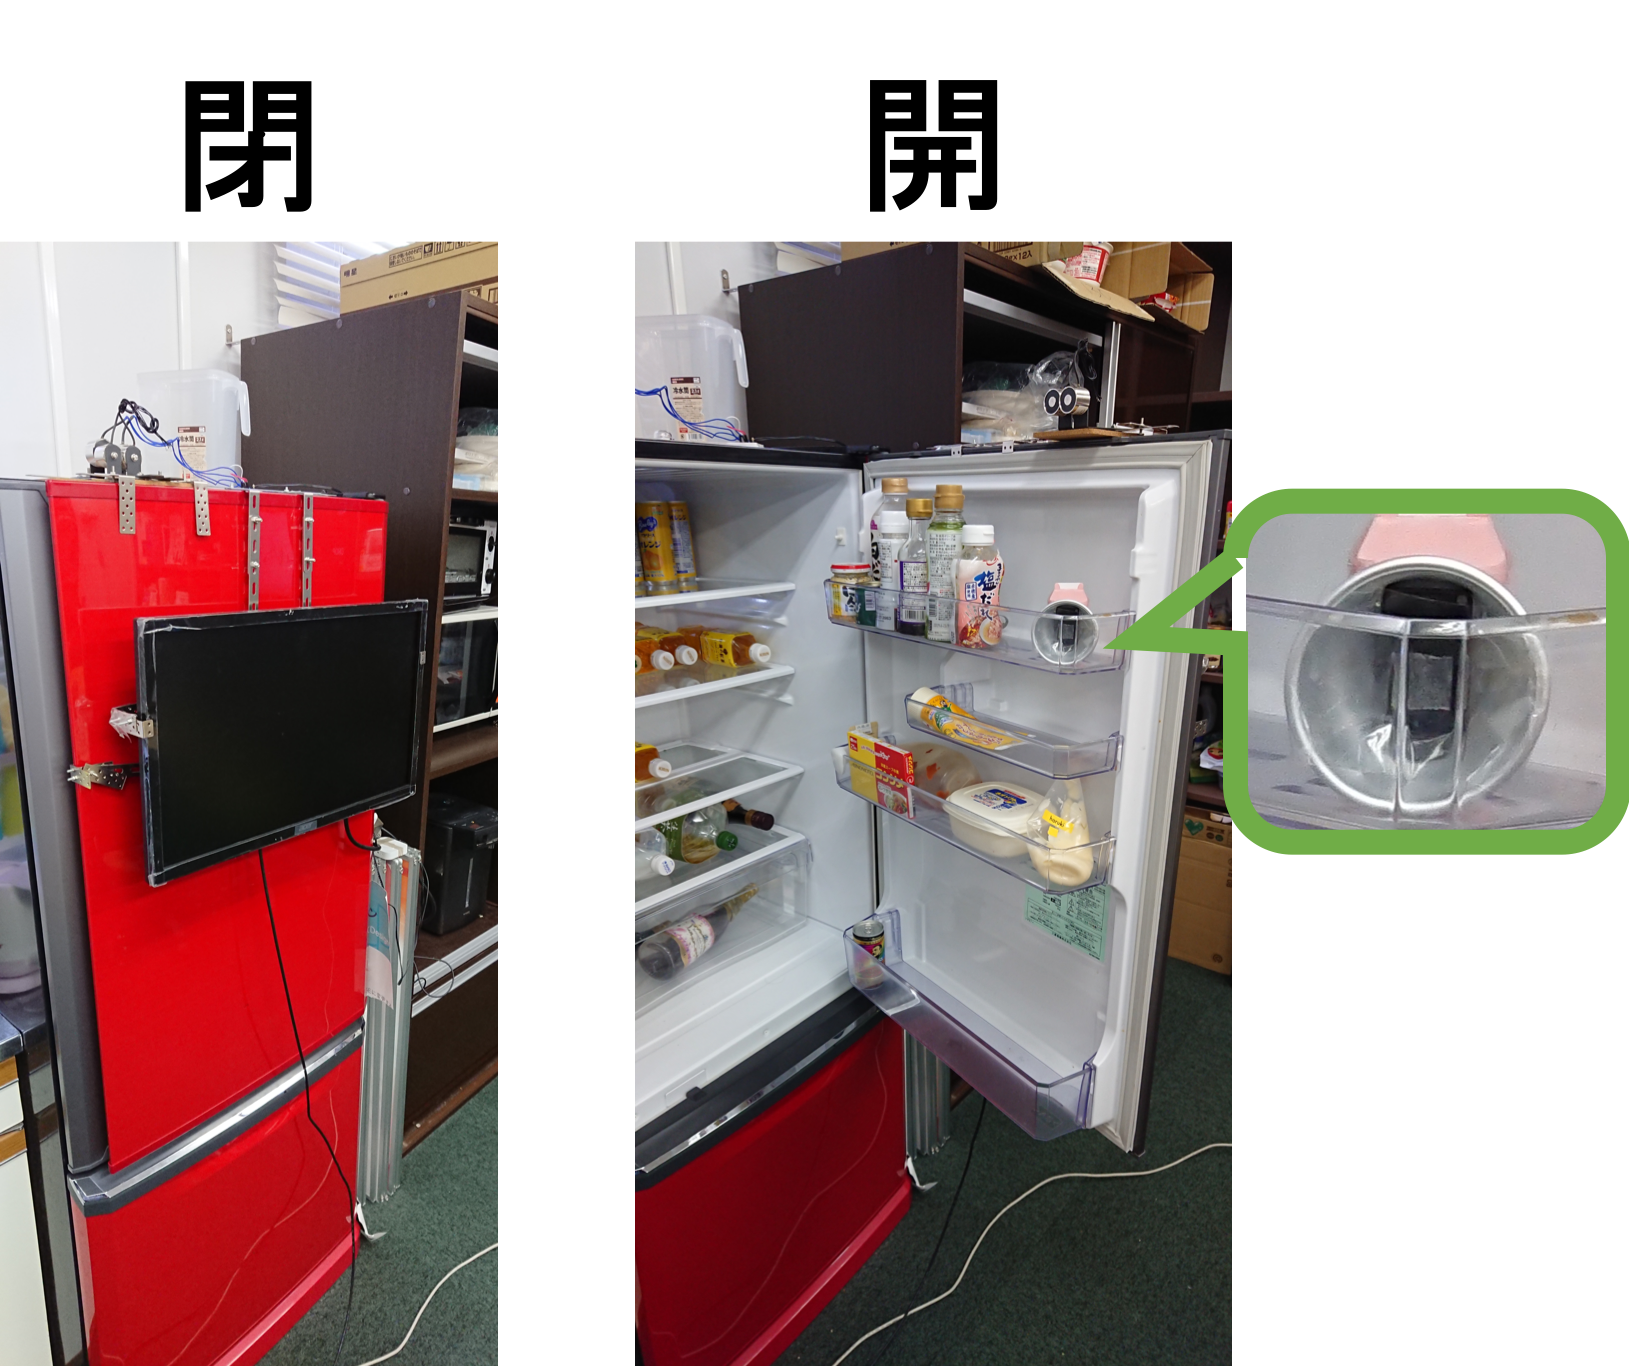
\includegraphics[width=7cm]{regisW2.png}
    \caption{冷蔵庫の状態と設置したビーコン}
    \label{freezer}
\end{figure}
\begin{figure}[ht]
    \centering
    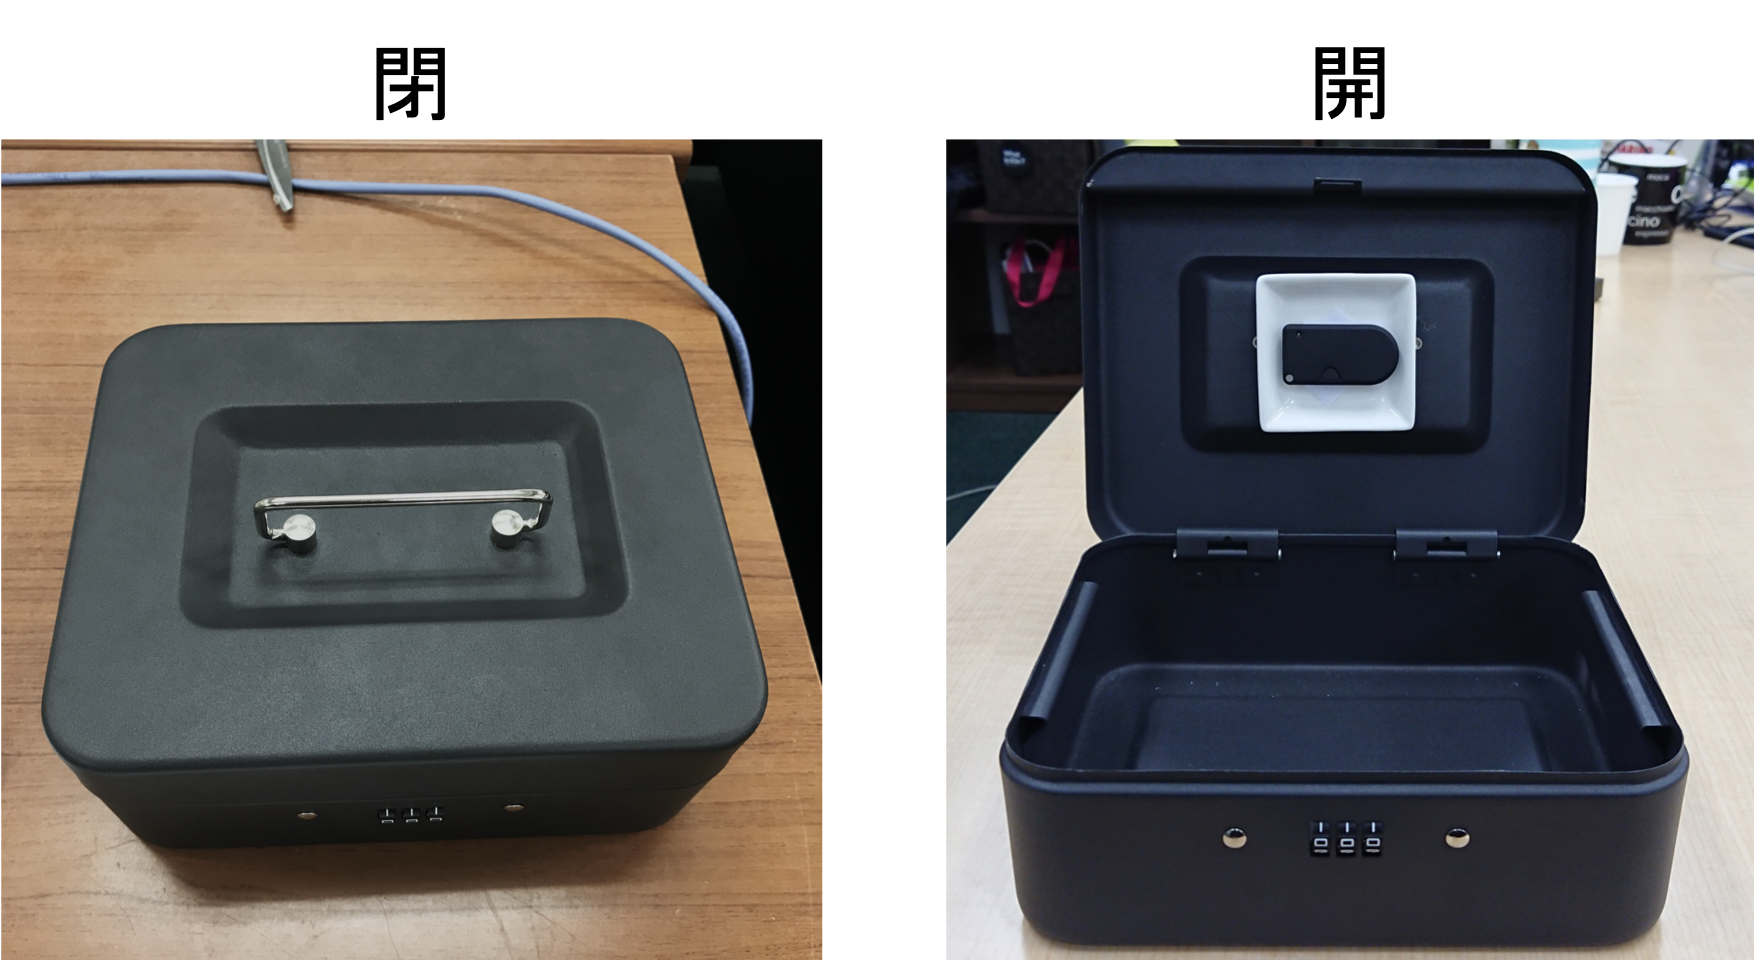
\includegraphics[width=7cm]{kinkoW.png}
    \caption{金庫の状態と設置したビーコン}
    \label{safe}
\end{figure}
\begin{figure}[ht]
    \centering
    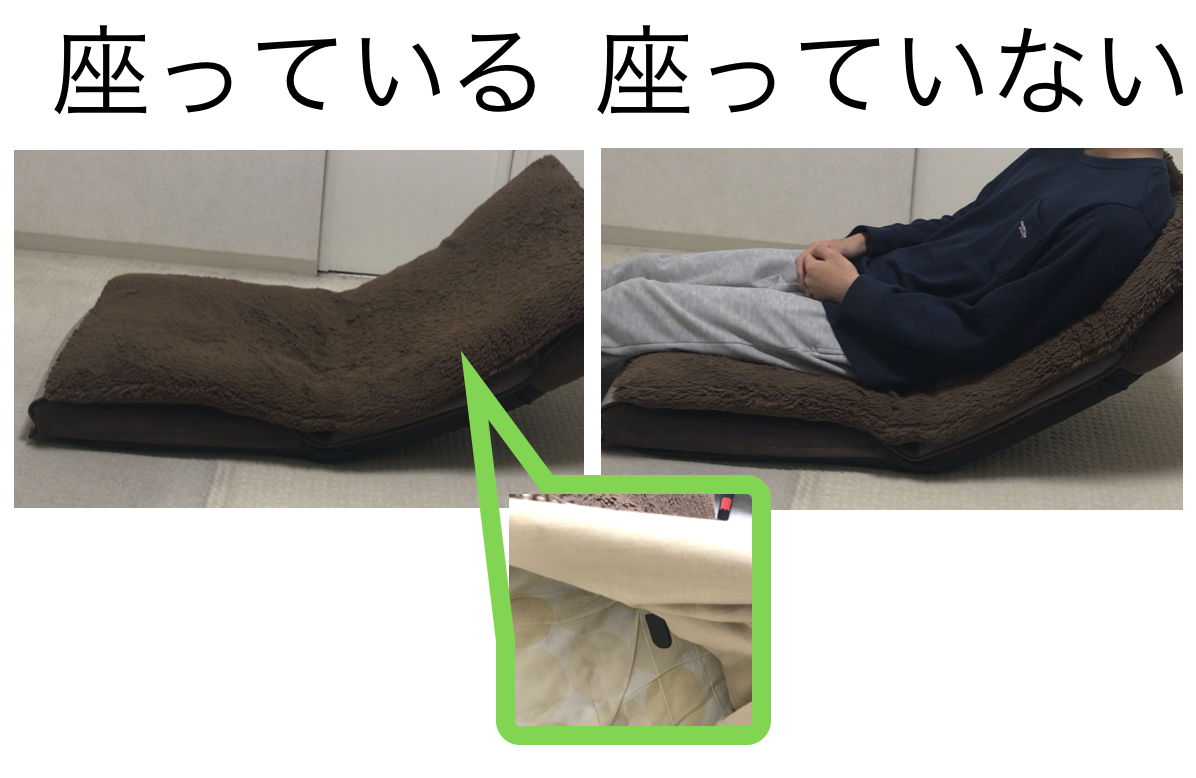
\includegraphics[width=8cm]{zaisuW.png}
    \caption{座椅子の状態と設置したビーコン}
    \label{chair}
\end{figure}

BLEビーコンの状態変化による電波強度の変化を利用した研究に池田ら\cite{BLEpkpk}の研究がある.
この研究は複数あるBLEビーコンの中から一つを手でぱかぱかすことでそのBLEビーコンを特定出来るというものである.
モノの状態変化時にはこのぱかぱかと同じ状態になるため状態の推定が可能であると考えられる.




%ーーーーーーーーーーーーーーーーーーーーーーーーーーーーーーーーーーーーーーーーーーーーーーーーー
%ーーーーーーーーーーーーーーーーーーーーーーーーーーーーーーーーーーーーーーーーーーーーーーーーー

\subsection{電波強度のデータ収集対象及び前提}

本研究では受信機としてスマートフォンを使用するため, 専用のAndroidアプリケーション(図\ref{phoneApp})を作成し電波強度の情報を収集する.
その際BLEビーコンを識別するためのUUID, major, minorをBLEビーコンを設置する対象と紐付けし, どのBLEビーコンの値がどの対象物の物なのか把握できるようにしている.
またBLEビーコンの電波送信設定は小さな変化も検知可能にするため送信強度は0dBm, 送信間隔は100msと設定した.

\begin{figure}[ht]
    \centering
    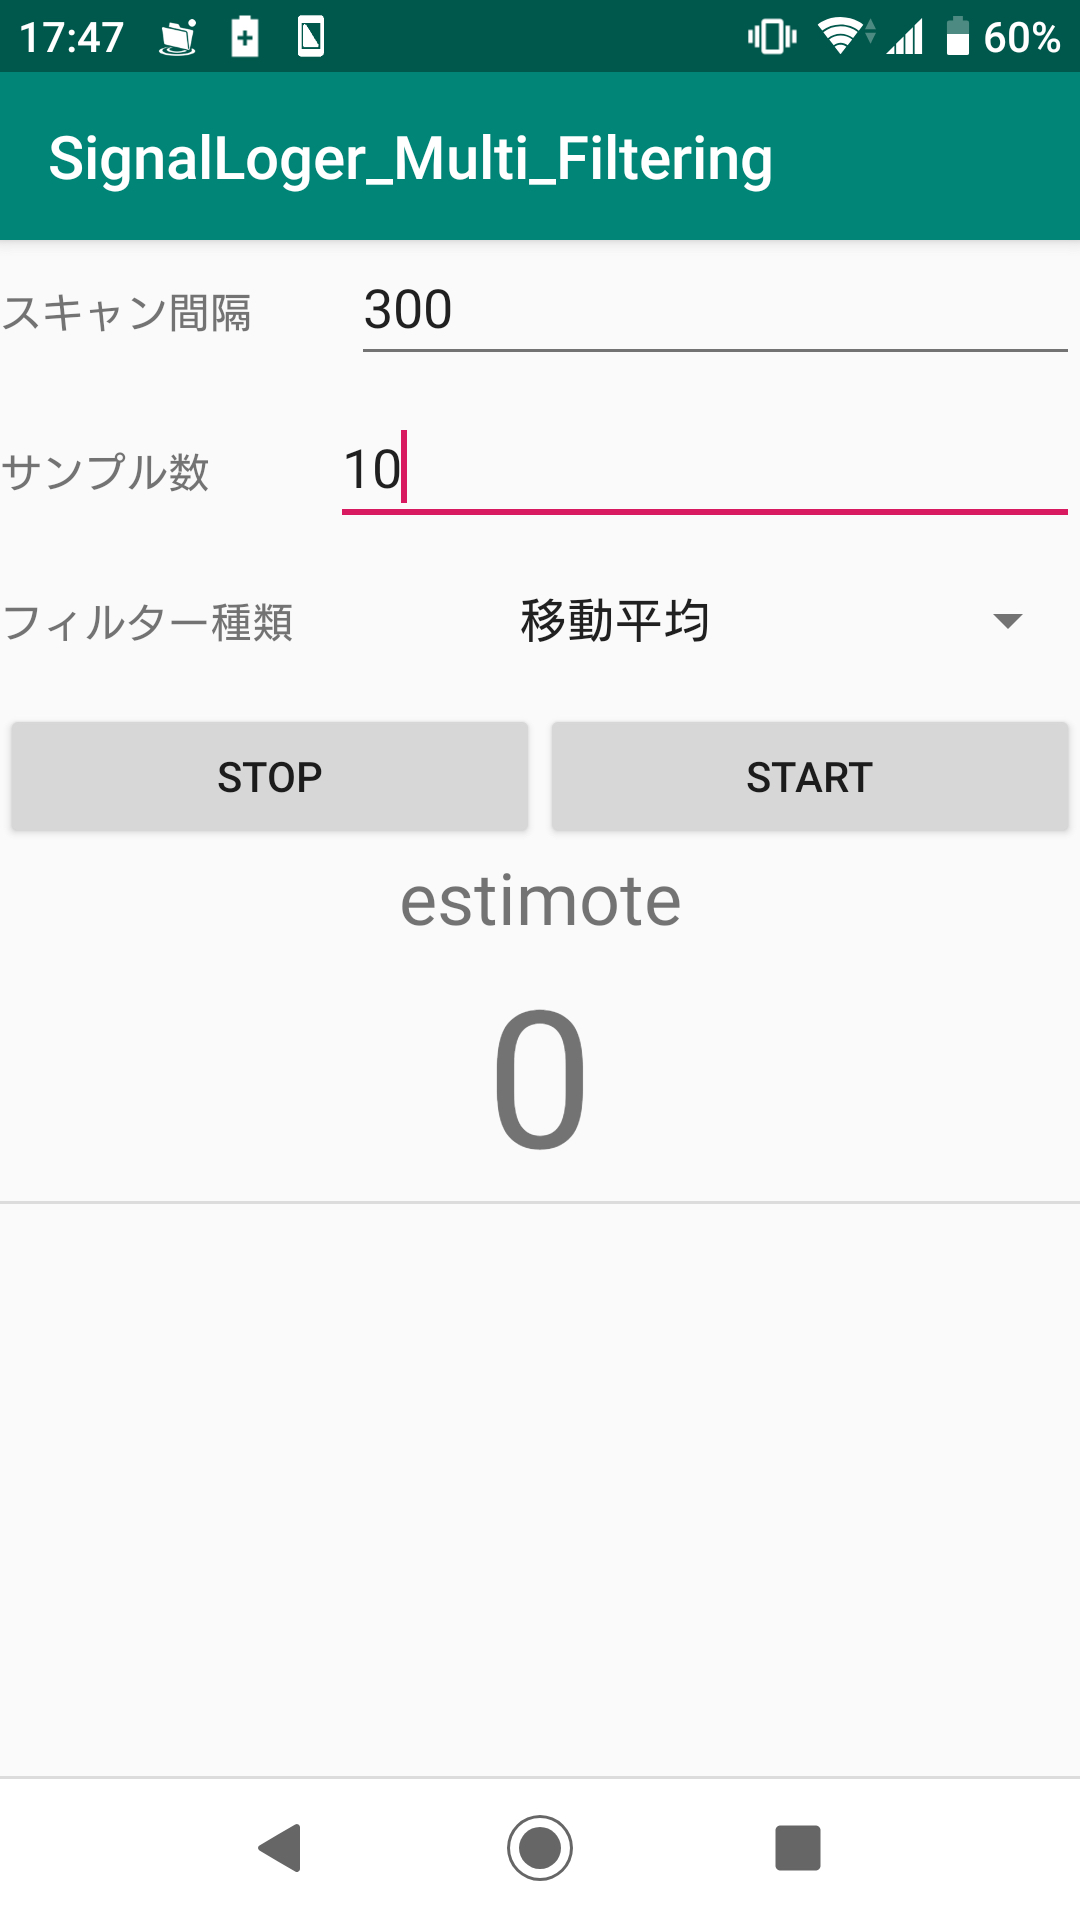
\includegraphics[height=5.5cm]{application.jpg}
    \caption{スマートフォン用アプリ}
    \label{phoneApp}
\end{figure}
% このアプリケsーションはBLEビーコンの受信電波強度を記録するだけではなく, リアルタイムでローパスフィルタの適用と安定センシング区間の判定及びそのネガポジ判定が可能である.




%ーーーーーーーーーーーーーーーーーーーーーーーーーーーーーーーーーーーーーーーーーーーーーーーーー
%ーーーーーーーーーーーーーーーーーーーーーーーーーーーーーーーーーーーーーーーーーーーーーーーーー


\subsection{BLEビーコン取り付け位置の検討}
BLEビーコンは取り付け位置や材質の違いにより対象物が状態変化した際の電波強度変化の仕方が異なる.
そこで, BLEビーコンの取り付け位置や付け方を変えることで電波強度変化の特徴を変える.
例えば箱型で蓋の開閉を行う金庫のようなものであれば, BLEビーコンを箱内部に設置する場合と蓋の裏に設置する場合が考えられる(図\ref{adapter}).
しかし, BLEビーコンを箱の底に取り付けた場合では状態変化による電波強度の変化があまり見られない.
これは箱の形からBLEビーコンの電波に指向性が持たされてしまい, 受信機の無い真上方向へ電波が飛んでしまったためと考えられる.

さらに, 対象の材質が電波を通しやすいために状態変化しても電波強度に大きな変化が現れないモノもあるため, 図\ref{adapter}のように電波に指向性をもたせるアダプタを取り付けることで電波強度にはっきりとした変化が出るようにする.
この指向性アダプタとはパラボラアンテナのような形状の金属や陶器のことを指し, これを取り付けることで電波が拡散せず収束して一方向のみへ飛ぶようになる.
その結果, 特定の方向に向かって飛ぶ電波が強まり, 状態変化によって電波強度に大きな変化が現れるようになる.

図\ref{transform-data}にそれぞれの取り付け方による金庫開閉時の電波強度の波形を示す.
この図にはそれぞれ開いている状態と閉じている状態の正解ラベルをつけている.
BLEビーコンを金庫内部の底につけた場合にはあまり大きな変化は見られず, 蓋の裏側にBLEビーコンを設置した場合では大きな変化が見られる.
さらに指向性アダプタをつけた場合にはよりくっきりと電波強度に差が現れることがわかる.
このようにして状態推定対象に合わせてBLEビーコンの取り付け方を工夫し, 状態変化によって大きく電波強度を変化させ状態推定を行う.


% 図の挿入
\begin{figure}[ht]
    \centering
    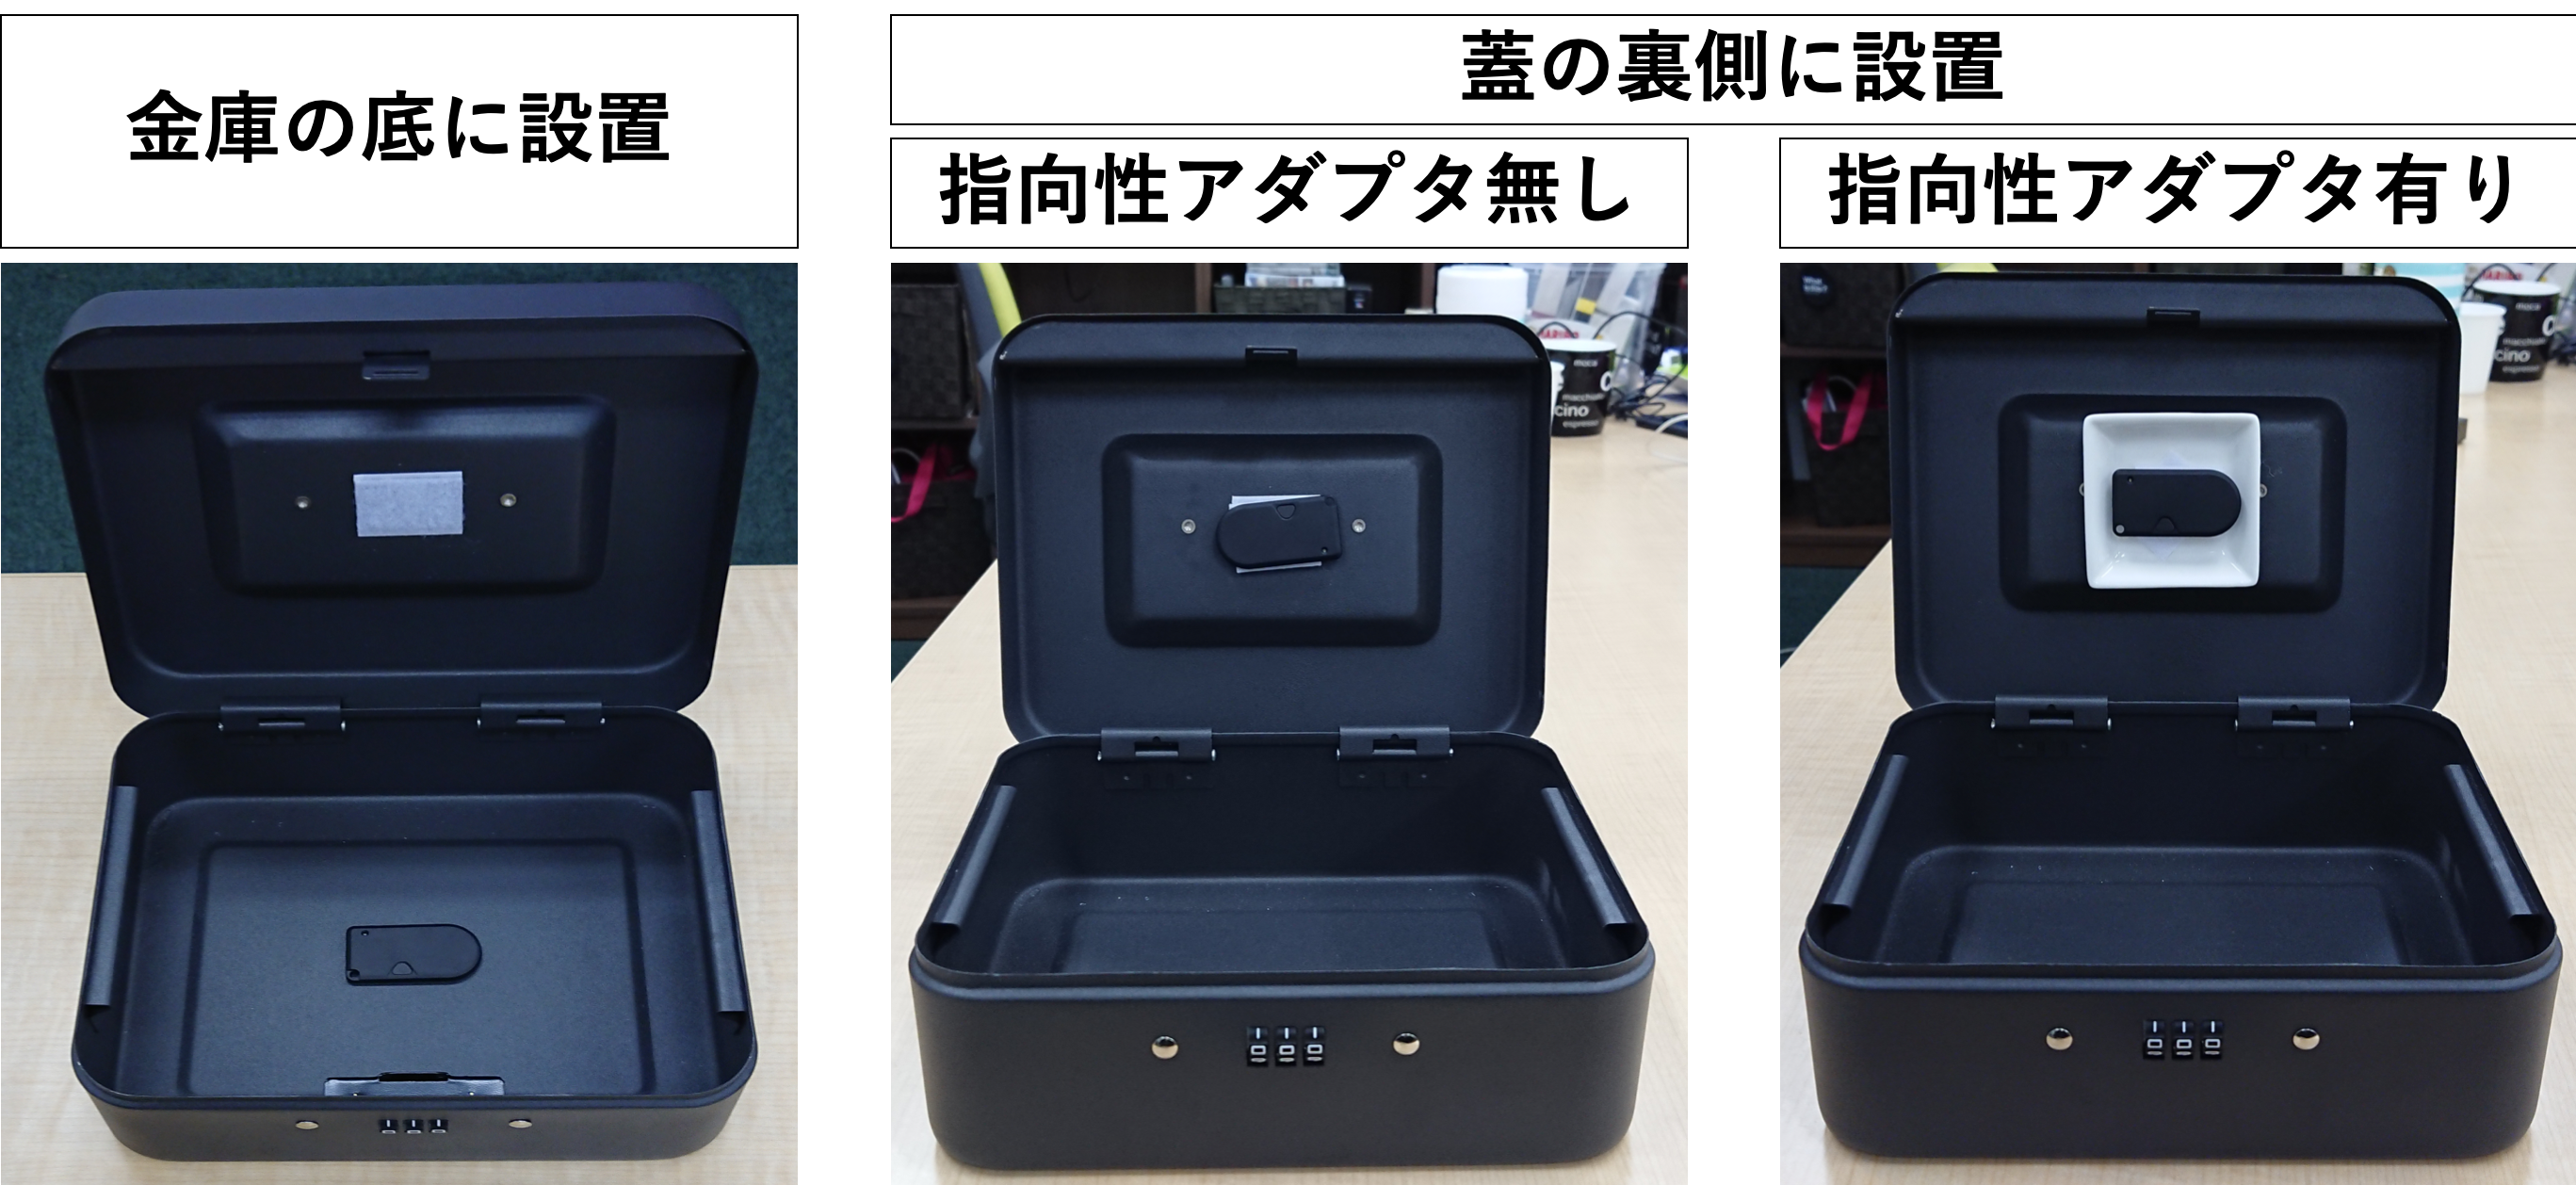
\includegraphics[width=8cm]{adapta_compare2.png}
    \caption{指向性アダプタ有り無しの画像}
    \label{adapter}
   \end{figure}


% 図の挿入
\begin{figure}[ht]
    \centering
    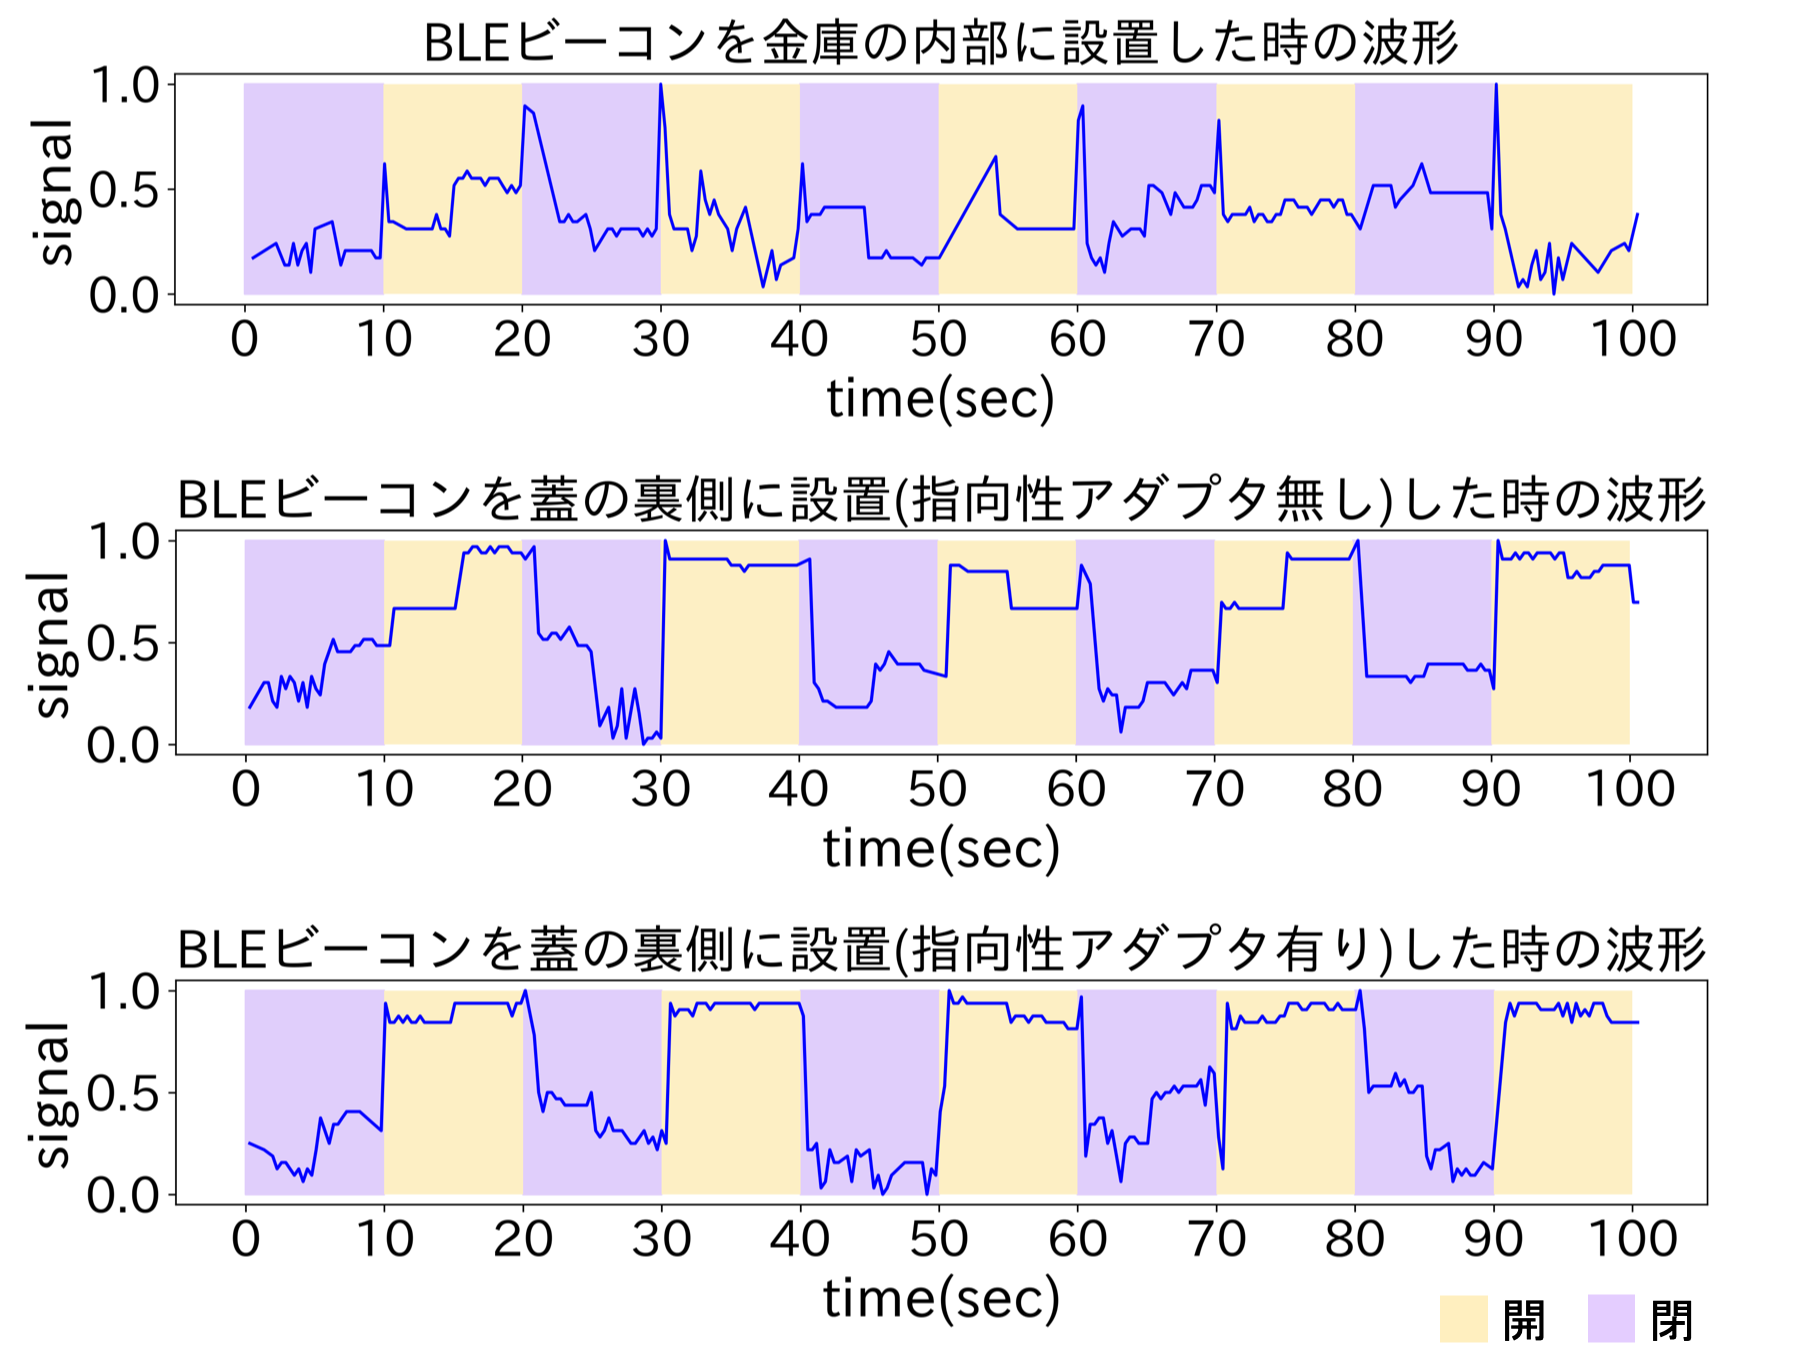
\includegraphics[width=8cm]{in-out.png}
    \caption{ビーコン取り付け位置毎の電波強度変化}
    \label{transform-data}
\end{figure}
%ーーーーーーーーーーーーーーーーーーーーーーーーーーーーーーーーーーーーーーーーーーーーーーーーー
%ーーーーーーーーーーーーーーーーーーーーーーーーーーーーーーーーーーーーーーーーーーーーーーーーー

\subsection{状態推定アルゴリズム}
本手法ではBLEビーコンから発せられる電波をスマートフォンで受信し, その受信強度の値から状態を推定する.
図\ref{bank-opcl}は金庫の開閉を行ったときの電波強度の値に, 移動平均を用いたローパスフィルタをかけて小さな揺らぎを除去したグラフである.

\begin{figure}[t]
 \centering
 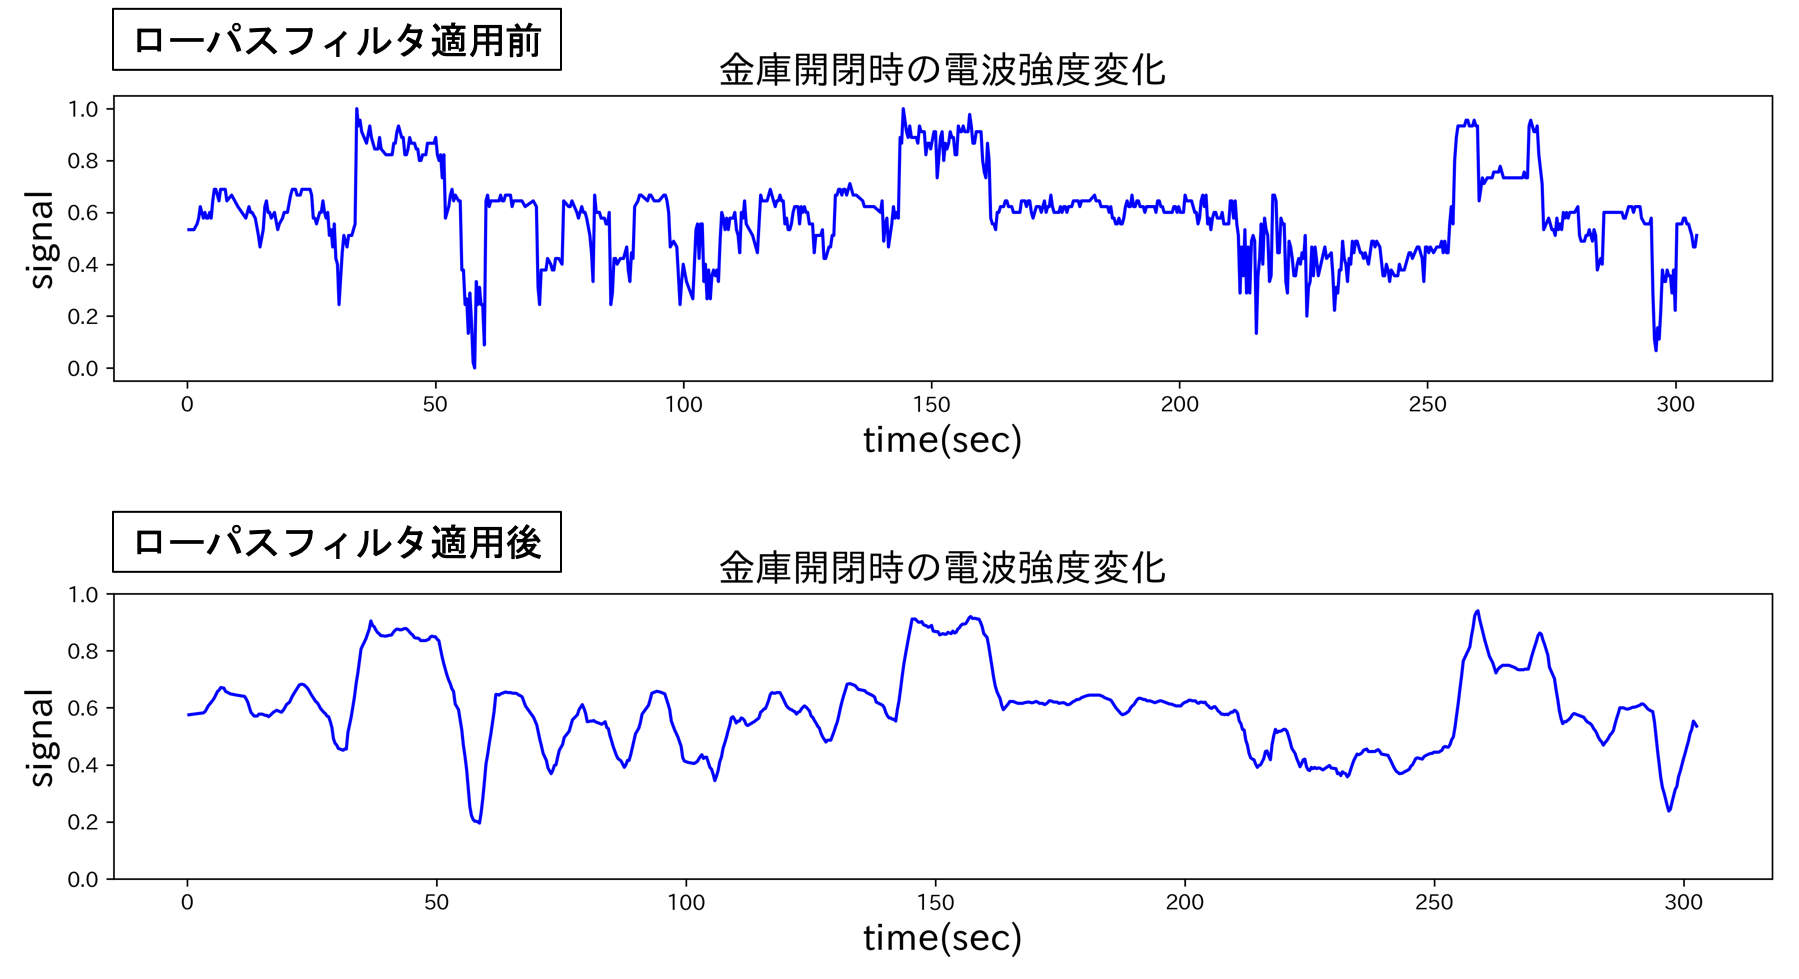
\includegraphics[width=8cm]{lowpath_compare.png}
 \caption{ローパスフィルタ適用前後の電波強度グラフ}
 \label{bank-opcl}
\end{figure}

収集した電波強度の値を正規化し0から1の値に変換する.
一時的な障害物があった場合や状態変化に際した人間の影響などにより電波強度にローパスフィルタでは除去しきれない揺らぎが発生する事があるため, 梶ら\cite{sensing-area}が提案している安定センシング区間という概念を利用し推定精度の高精度化を図る.
安定センシング区間とは一定時間以上センシングが安定して行えている区間を指す.
本手法はデータをスマートフォンで収集した後に適用可能なオフライン手法である.


\subsubsection{安定センシング区間}
本手法では推定対象物の移動も考慮するため, 安定センシング区間の判定に吉澤らの提案手法\cite{ips-chube}内で利用されているεチューブを利用する.
物体が状態変化をせず移動した場合, 徐々に電波強度は変化するため単純な閾値を用いた推定では長距離移動し電波強度が大幅に減衰した際に誤判定が起こってしまう.
εチューブは一つ前の電波強度の値と現在の電波強度の値を使用し, 現在の値が一つ前の値の上限・下限の閾値範囲内に収まっているかどうかで判定を行い, 一定時間以上閾値内に収まっていた場合にそこを安定センシング区間とする.
この時の上限・下限閾値を今回使用したBLEビーコンの特徴や推定対象に合わせ定める.
% 図の挿入
\begin{figure}[b]
    \centering
    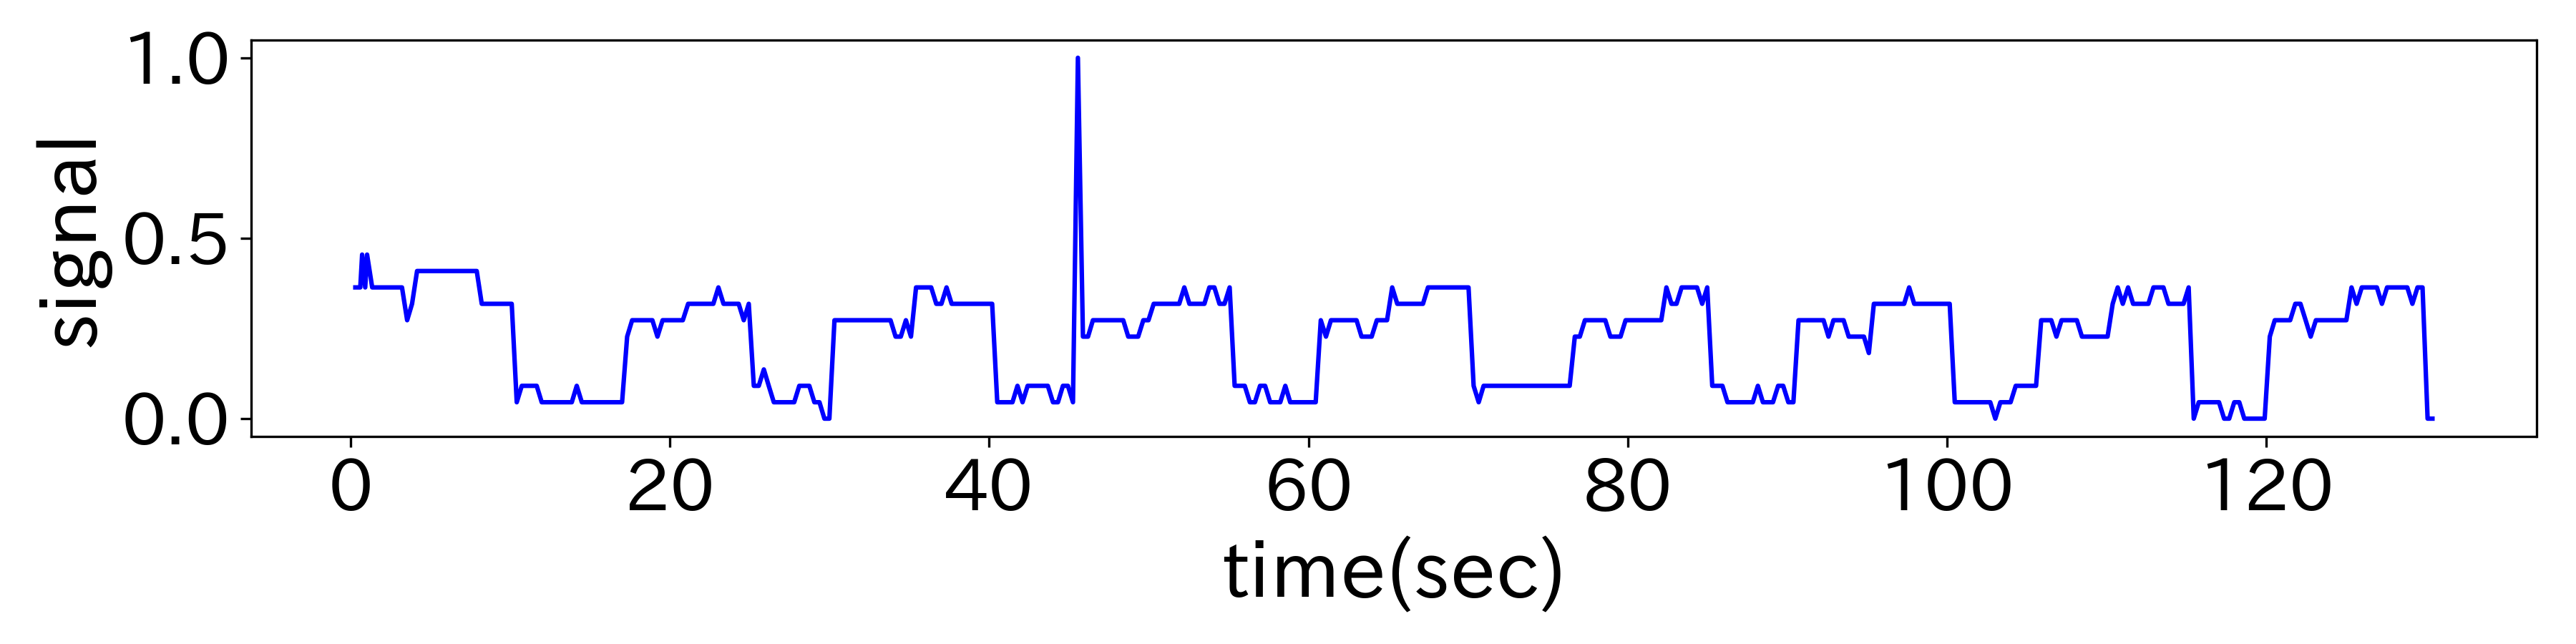
\includegraphics[width=8.5cm]{bokoboko.png}
    \caption{BLEビーコンをただ置いて測定した電波強度グラフ}
    \label{nomal-data}
\end{figure}

%@@@@@@@@@@@@@@@@@@@@@@@@@@@@@@@@
図\ref{nomal-data}はBLEビーコンをただ置いた状態での電波強度の値にローパスフィルタを適用したグラフであり, ここからBLEビーコンの電波は周期的に電波強度の変化が見られることがわかる.
このBLEビーコン特有の周期的な強度変化により安定センシング区間の判定が不安定になることがあるため, 適切な閾値を設定する必要がある.
対象の状態変化による電波強度の変化とBLEビーコン特有の電波強度の変化を考慮して動的に閾値を設定する.

%pythonプログラムの説明
オフラインプログラムでは最初に受信電波強度とその受信時間が記録されたファイルからデータを読み込む.
読み込んだ受信電波強度の数値は0〜1の値に正規化し, ローパスフィルタをかけてノイズを取り除く.
次に安定センシング区間を見つけるため受信電波強度の時系列データに対してεチューブを適用する.
εチューブは時系列に並んだデータを走査し, 予め設定しておいた閾値内に受信電波強度の値が収まっているか確認する.
もし閾値を超えた場合は, 超える直前の受信電波強度±X(Xは任意の値)の値を新しい閾値として設定する.
これを繰り返し安定センシング区間の判定が終わったら, 最後に見つけたそれぞれの安定センシング区間がネガティブな状態かポジティブな状態か判定を行う.
判定は, 各安定センシング区間の受信電波強度の平均値が受信電波強度の中央値に0.1を足した値より大きいか小さいかで判定を行う.


%@@@@@@@@@@@@@@@@@@@@@@@@@@@@@@@@@@
% 図の挿入
% \begin{figure}[ht]
%  \centering
%  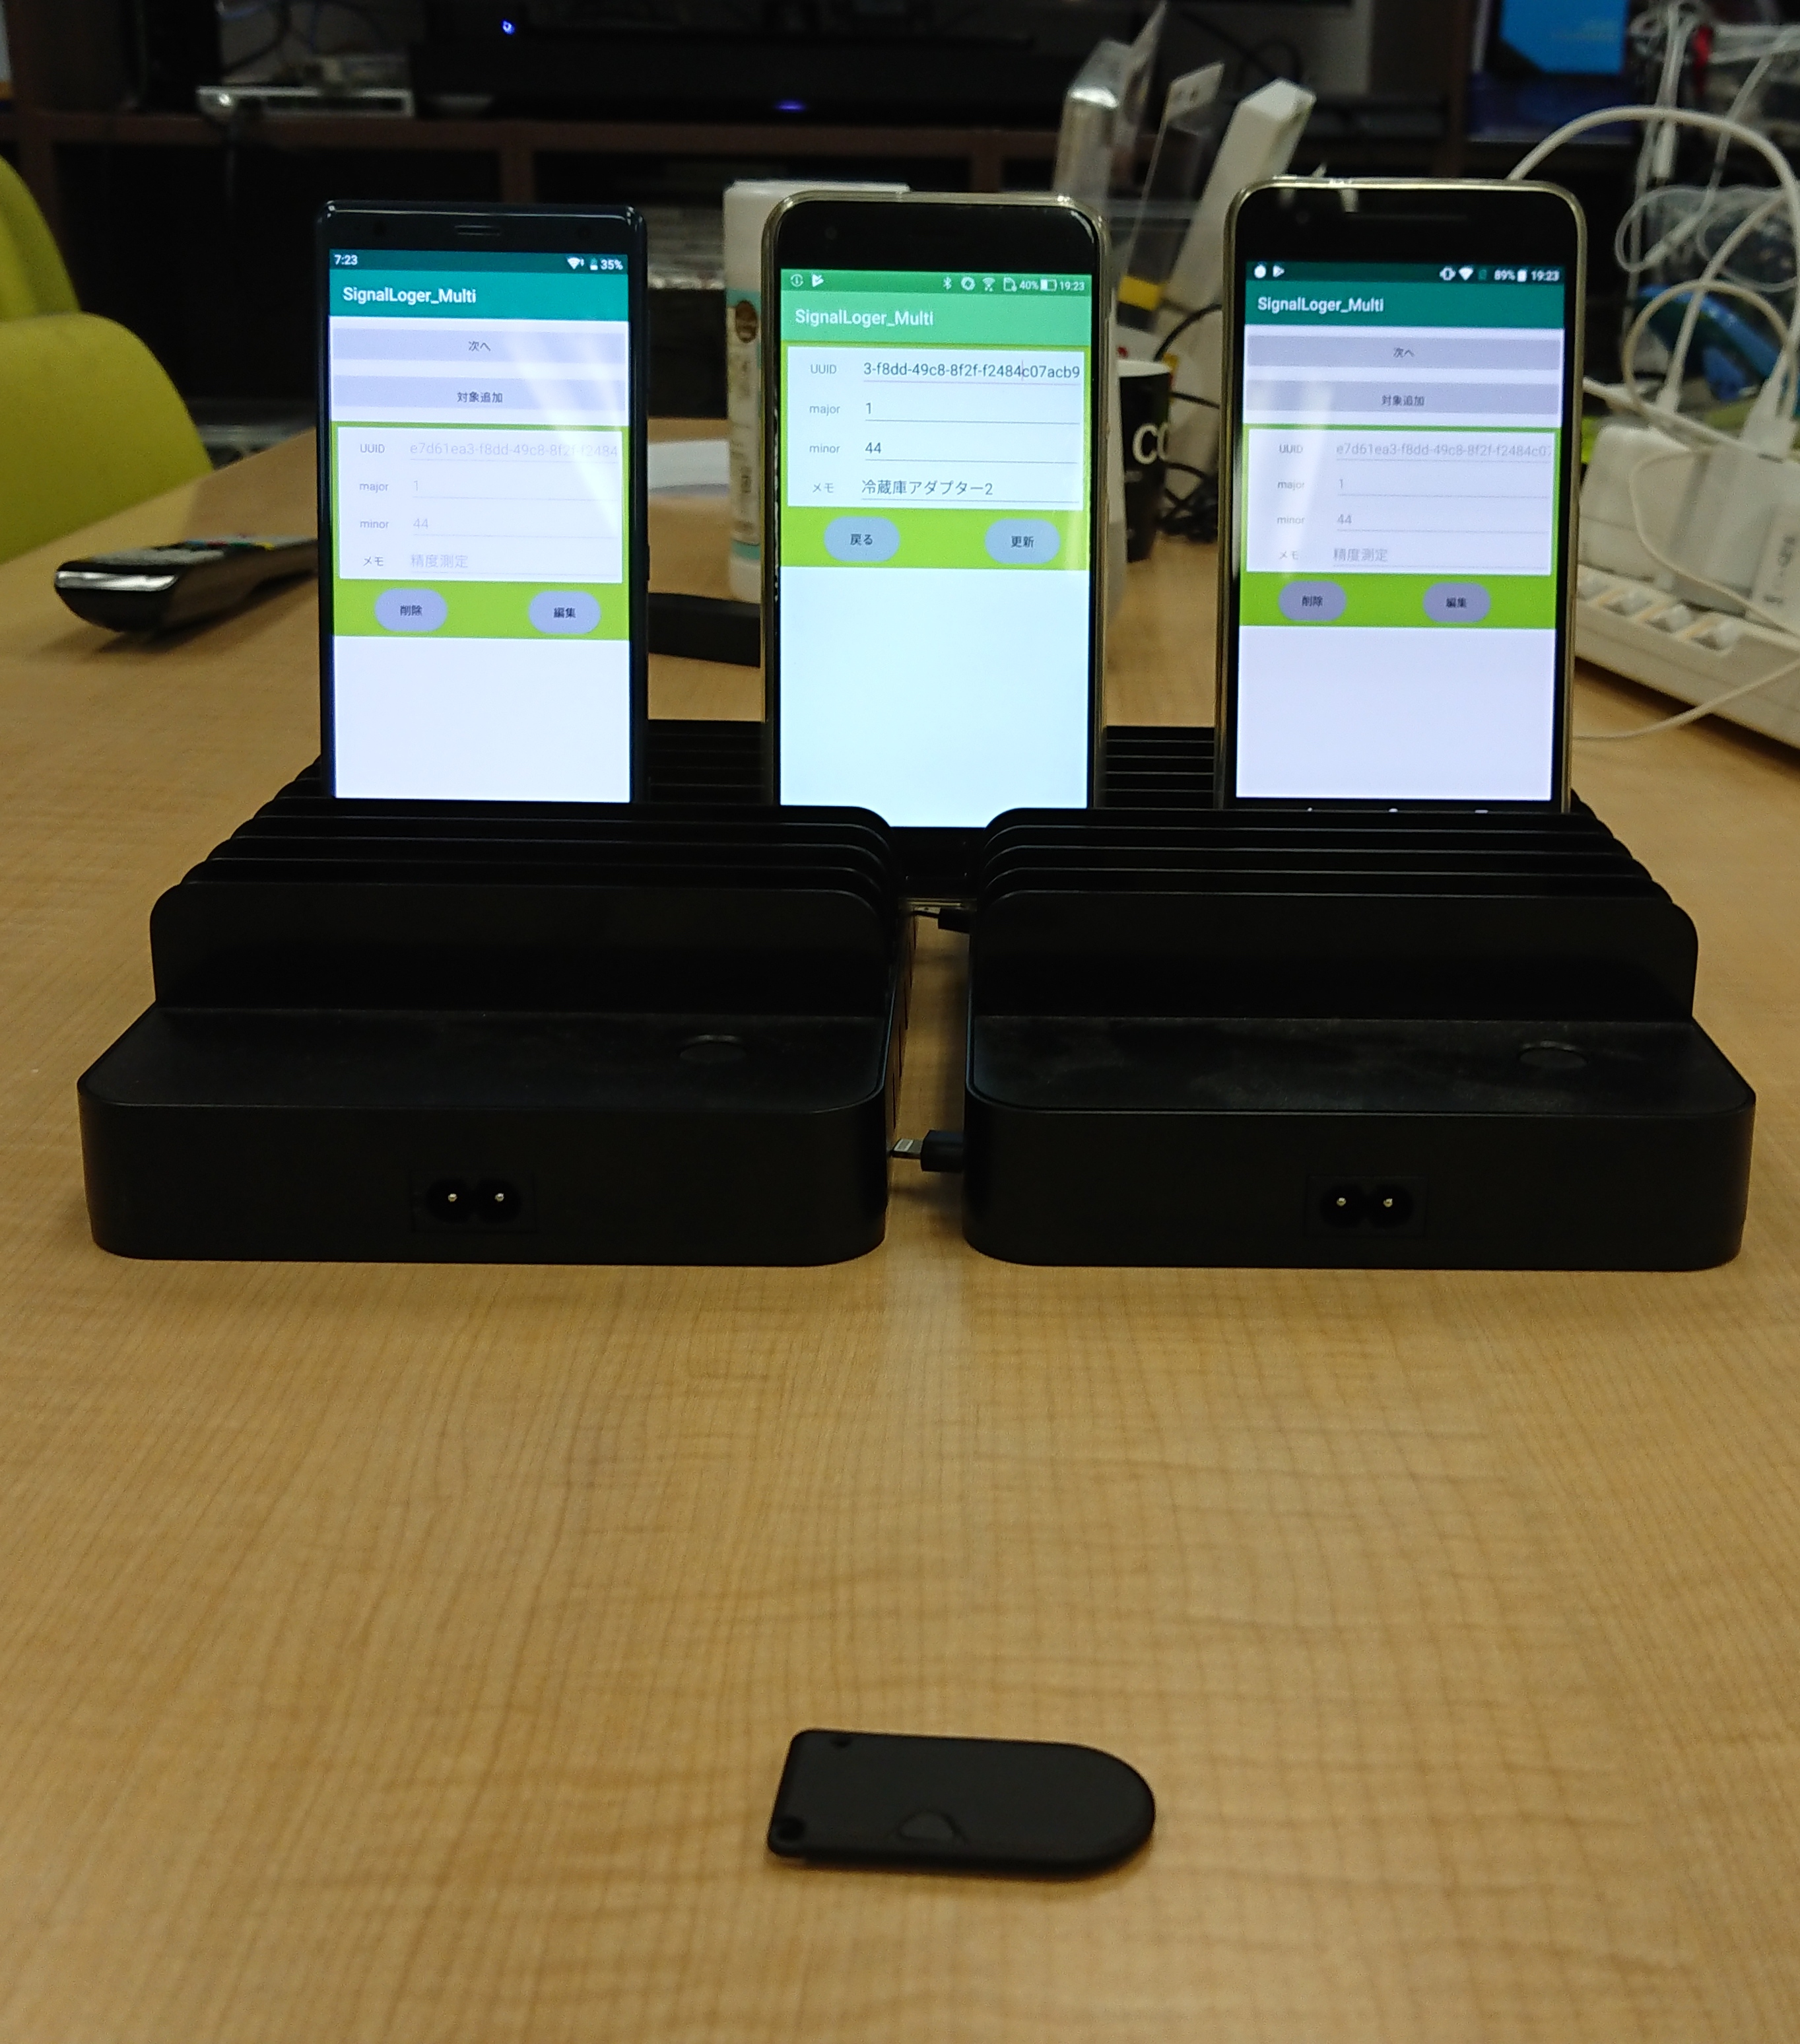
\includegraphics[width=7.5cm]{compare.jpg}
%  \caption{BLEビーコンただおきのデータ}
%  \label{compare}
% \end{figure}


\subsubsection{状態変化の推定}
推定結果の状態をネガティブな状態とポジティブな状態の2つの状態とする.
ポジティブな状態とはBLEビーコンが外に出ていて電波の受信がしやすく、電波強度の値が高い状態の事を指す. 具体的には金庫の開閉であれば開いてる状態である.
ネガティブな状態とはBLEビーコンが外に出ておらず電波の受信が難しく、電波強度の値が低い状態の事を指す. 具体的には金庫の開閉であれば閉じてる状態である.
判定された安定センシング区間内の平均値をそれぞれ求め,すべての安定センシング区間の平均値の中央値より高いか低いかでネガティブポジティブの判定を行う.



%ーーーーーーーーーーーーーーーーーーーーーーーーーーーーーーーーーーーーーーーーーーーーーーーーー
%ーーーーーーーーーーーーーーーーーーーーーーーーーーーーーーーーーーーーーーーーーーーーーーーーー


\section{評価実験}

本稿で提案した手法の推定精度を確かめるため, いくつかのモノへBLEビーコンを設置し評価実験を行った.
BLEビーコンを設置する対象は, 冷蔵庫, 金庫, 座椅子とし, 金庫と座椅子については移動を考慮した状態変化に対し推定精度を測定した.
評価の方法は開閉などの状態変化をランダムな間隔で行い, その推定結果と正解ラベルを比べて正答率を算出して行う.

\subsection{実験端末の選定}

\begin{figure}[ht]
    \centering
    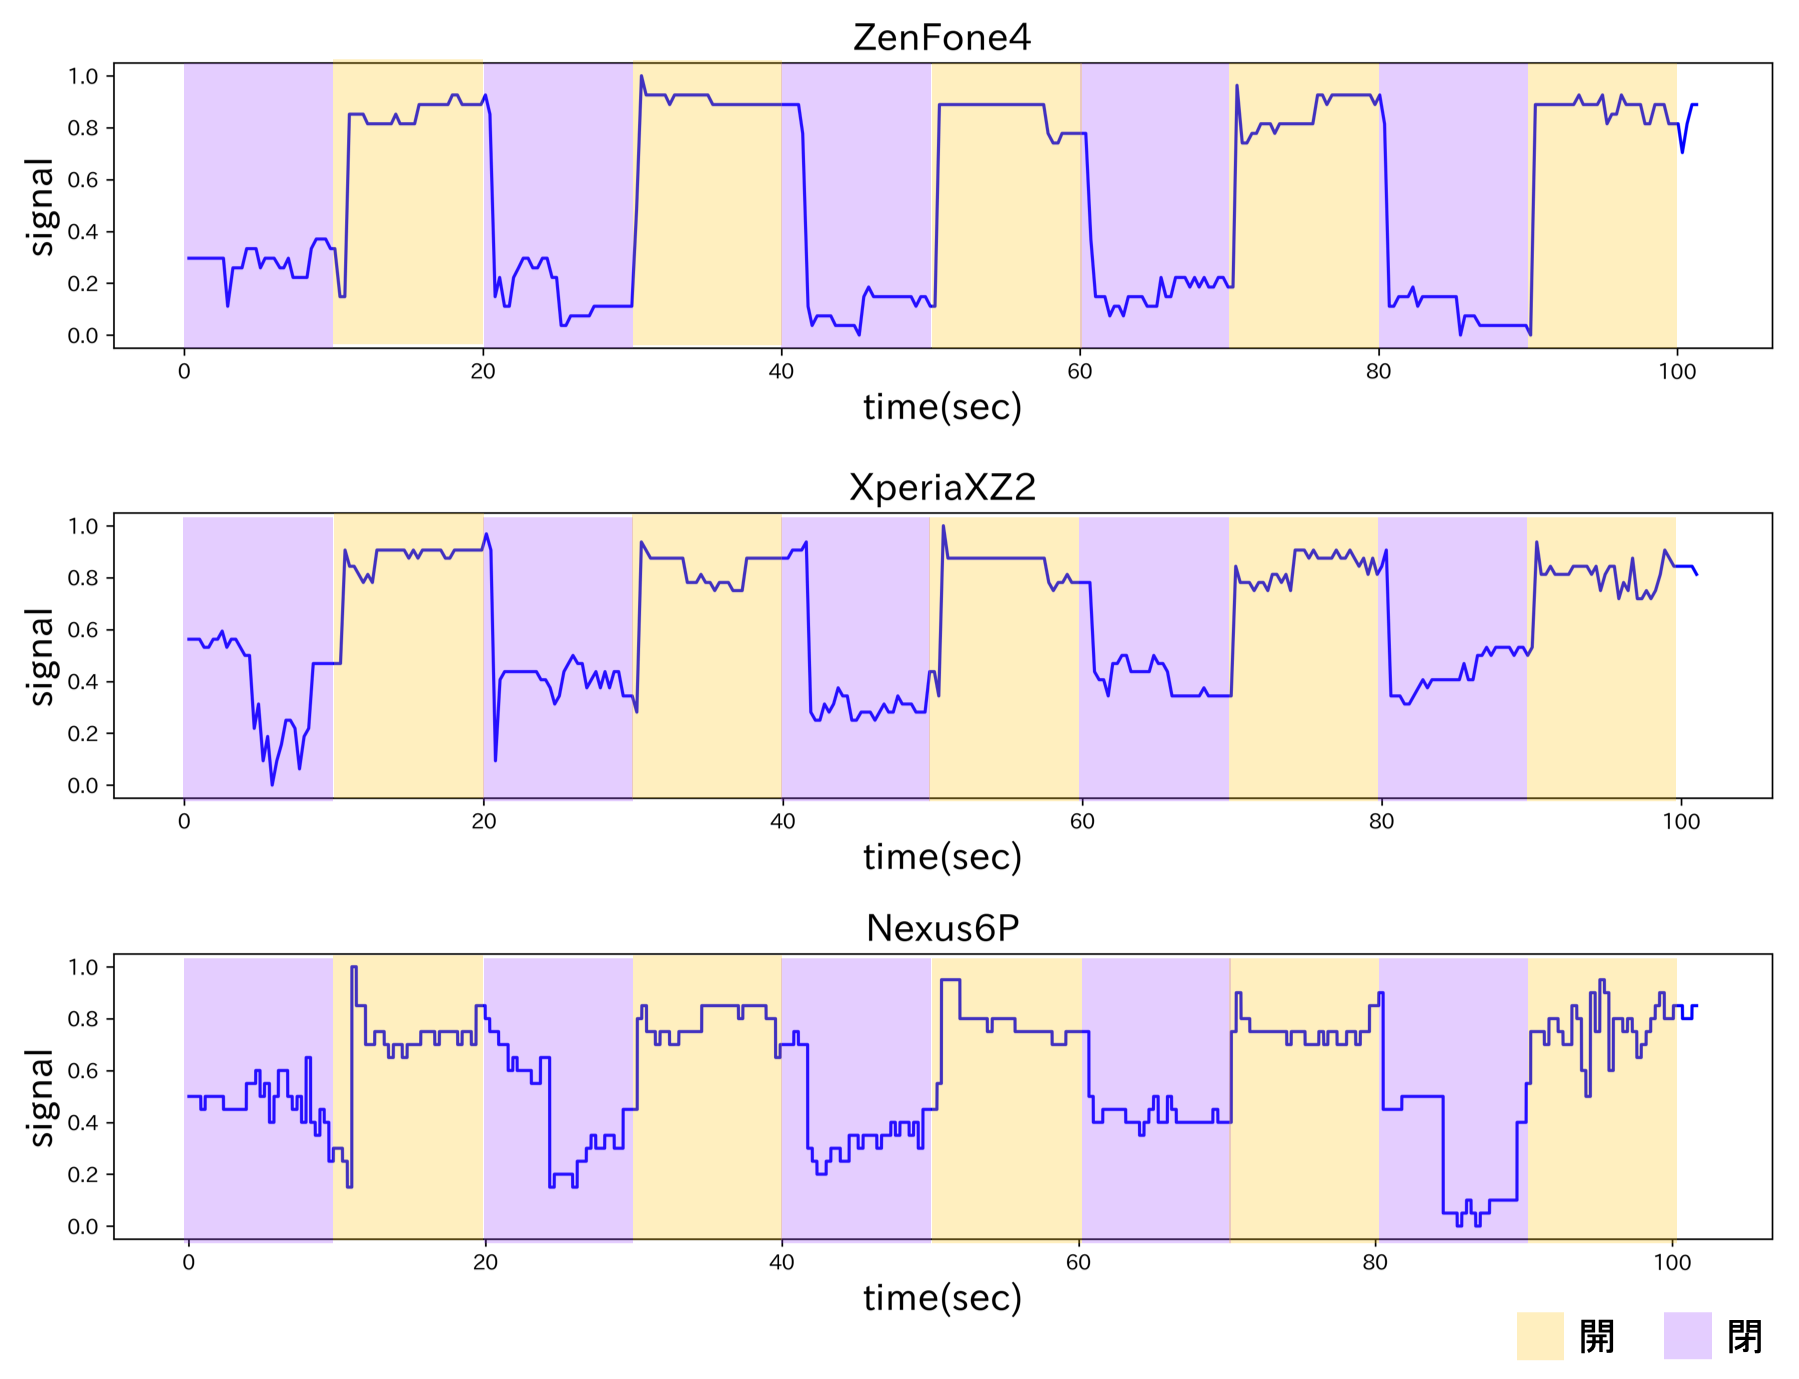
\includegraphics[width=8cm]{mix.png}
    \caption{機種ごとの精度比較}
    \label{multi-data}
\end{figure}

Bluetoothのセンサ精度は端末毎に異なるため, 実験に用いる端末は変化を正しく捉えられる端末を使うのが望ましい.
そこで3機種を用意し, 同一環境下で金庫の蓋の開閉を行い測定精度の比較を行った.
今回用意した端末はXperiaXZ2, Nexus6P, ZenFone4である.
金庫開閉時の電波強度変化を各端末で収集し, その波形を比較した結果を図\ref{multi-data}に示す.
図の紫色の部分は蓋が閉まっていることを黄色の部分は蓋が開いていることを示している.
3機種の精度を比較した結果, Nexus6Pでは全体的に小さなノイズが発生しているがZenFone4とXperiaXZ2ではそれが少ないことを確認した.
また, XperiaXZ2とNexus6Pは測定開始直後は測定値が安定せず正しく変化を示せていないことを確認した.

本研究で提案する手法は電波強度の急激な変化と安定センシング区間の判定が重要となる.
そのため, 測定ノイズが少ないこと, きちんと変化が捉えられることが重要である.
以上の理由から本研究では一番ノイズが少なく, きちんと変化を捉えられるZenFone4を受信機として使用する.
また, 本研究では金庫などの移動を伴う比較的小さなモノにもBLEビーコンを取り付けるため, 使用するBLEビーコンはできるだけ小さい方が望ましい.
そのため使用するBLEビーコンは, 軽量・小型という理由からフォーカスシステムズ社のFCS1301\ref{beacon}を使用する.


\subsection{冷蔵庫の開閉における推定精度の測定}
図\ref{freezer}, 図\ref{refrigerator_position}のようにセンサと受信機を設置して評価実験を行った.
実験は日常の使用を模倣し, 冷蔵庫のドアを開けて, 中からペットボトルを取り出し, ドアを閉めるという動作をランダムな間隔で行い, その状態の変化を捉えることができるかで評価を行った.
この時電波強度の変化をはっきりさせるため3.2章で述べた指向性アダプタを取り付けた.
推定結果を図\ref{refrigerator_graph}に, 正解率の一覧を表\ref{refrigerator_fig}に示す.
図\ref{refrigerator_graph}の白色の範囲は安定センシング区間ではない状態を 緑色の範囲はネガティブな状態(ドアが閉まっている状態)を 赤色の範囲はポジティブな状態(ドアが開いている状態)を示している.

同様の実験を3回行った結果1回だけ不正解があり, 結果として全体の正解率は98.0%となった.
誤判定された400秒付近のグラフを見てみると他と比べて受信電波強度の変化が小さく, 安定センシング区間と判断されていないことが分かる.
このことから安定センシング区間を判定するパラメータを見直すことで誤判定を避けられると考える.

\begin{figure}[ht]
    \centering
    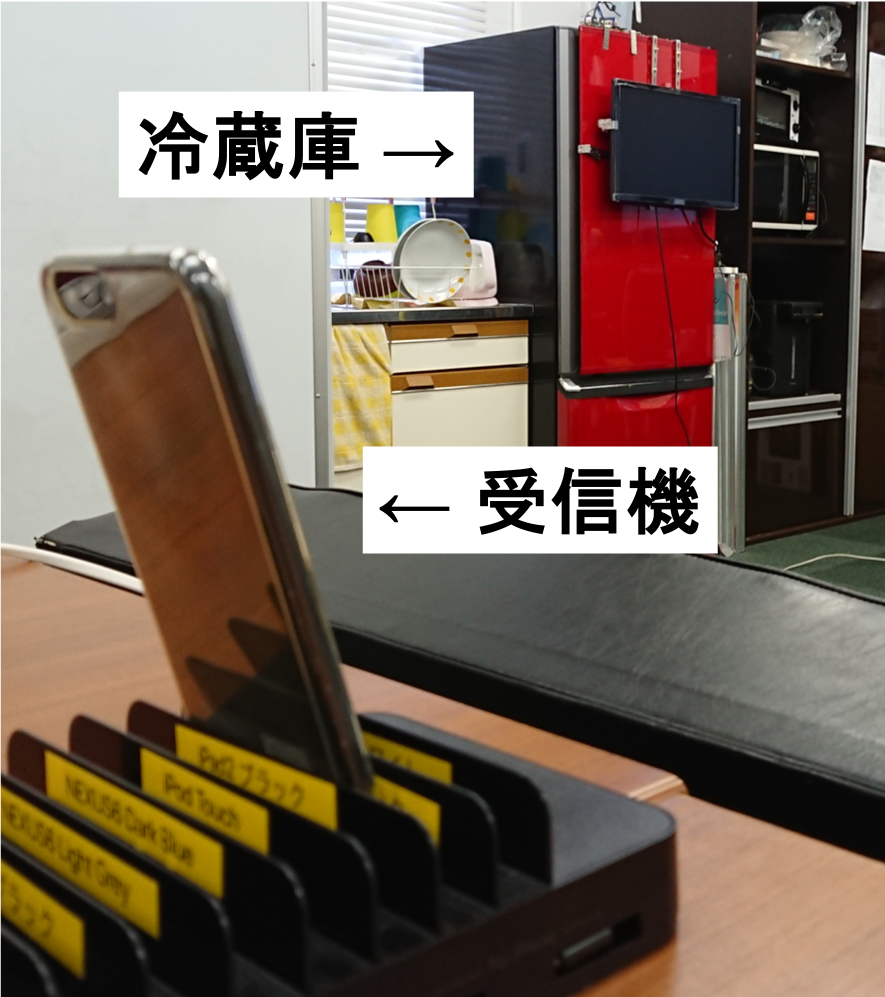
\includegraphics[height=5cm]{refrigerator_position.png}
    \caption{冷蔵庫と受信機の位置関係図}
    \label{refrigerator_position}
\end{figure}

\begin{figure}[ht]
    \centering
    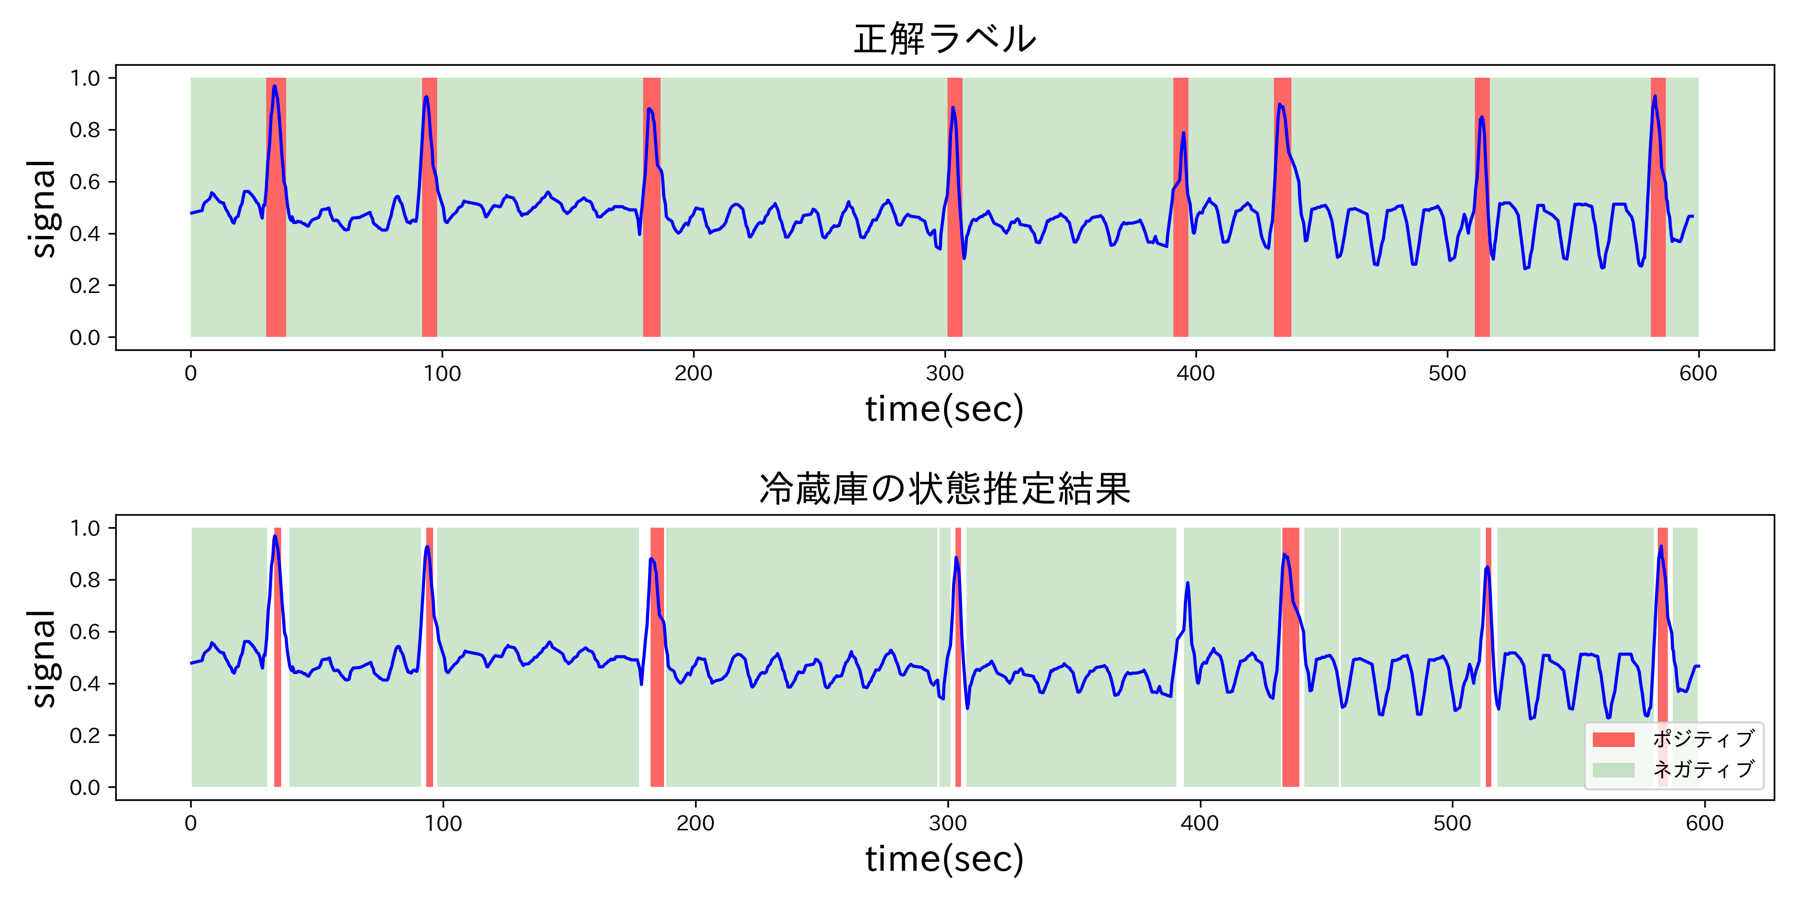
\includegraphics[width=8cm]{refrigerator_graph.png}
    \caption{冷蔵庫の状態推定結果グラフ}
    \label{refrigerator_graph}
\end{figure}



%@@@@@@@@@@@@@@@@@@@@
%  ポジティブな状態だけ検出できた割合の結果 ではなくネガティブポジティブ両方の検出数から割合を出すべきでは????
%@@@@@@@@@@@@@@@@@@@@
\begin{table}[htb]
    \begin{center}
        \caption{冷蔵庫の開閉における状態推定精度}
        \label{refrigerator_fig}
        \begin{tabular}{|c|c|c|c|} \hline
        試行回数 & 正答率 & 正解数 & 不正解数 \\ \hline
        1 & 94.1% & 16 & 1 \\ \hline
        2 & 100% & 17 & 0 \\ \hline
        2 & 100% & 17 & 0 \\ \hline \hline
        累計正解率 & \multicolumn{3}{c|}{98.0%} \\ \hline
        \end{tabular}
    \end{center}
\end{table}



\subsection{金庫の開閉における推定精度の測定}
図\ref{safe}, 図\ref{kinko_position}のようにセンサと受信機を設置して評価実験を行った.
金庫は図\ref{kinko_position}に赤丸で示したように3箇所の場所に移動させて蓋の開閉を行い, 推定中にモノの移動が行われても状態推定が可能かを確かめた.
推定結果を図\ref{kinko_graph}に, 正解率の一覧を表\ref{kinko_fig}に示す.
図\ref{kinko_graph}の白色の範囲は安定センシング区間ではない状態を 緑色の範囲はネガティブな状態(蓋が閉まっている状態)を 赤色の範囲はポジティブな状態(蓋が開いている状態)を示している.
また, 図中の番号は図\ref{kinko_position}内の番号と対応している.

同様の実験を3回行った結果, 3回とも正しく蓋の開閉を検知することができた.
しかし, 2番の場所での推定結果を見てみると, 蓋が閉まった後も数秒間蓋が開いていると推定されてしまっている.
% 蓋が閉まって電波強度が弱まった160秒付近のグラフを見てみると変化終了後のグラフがほぼ真横に一直線になっている.
これはBLEビーコン特有の周期的な電波強度の変化が安定センシング区間の判定に影響されないよう少し大きめの閾値を取ったため, この2の開ける動作後の電波強度がこの下限閾値を超えられなかった.
このため蓋の開閉が終わった後もポジティブな状態と判定されてしまい誤判定が発生したのだと考えられる.
また, このことから冷蔵庫と同様に安定センシング区間を判定する閾値などのパラメータを見直すことでこのような誤判定は避けられるのではと考えられる.

\begin{figure}[ht]
    \centering
    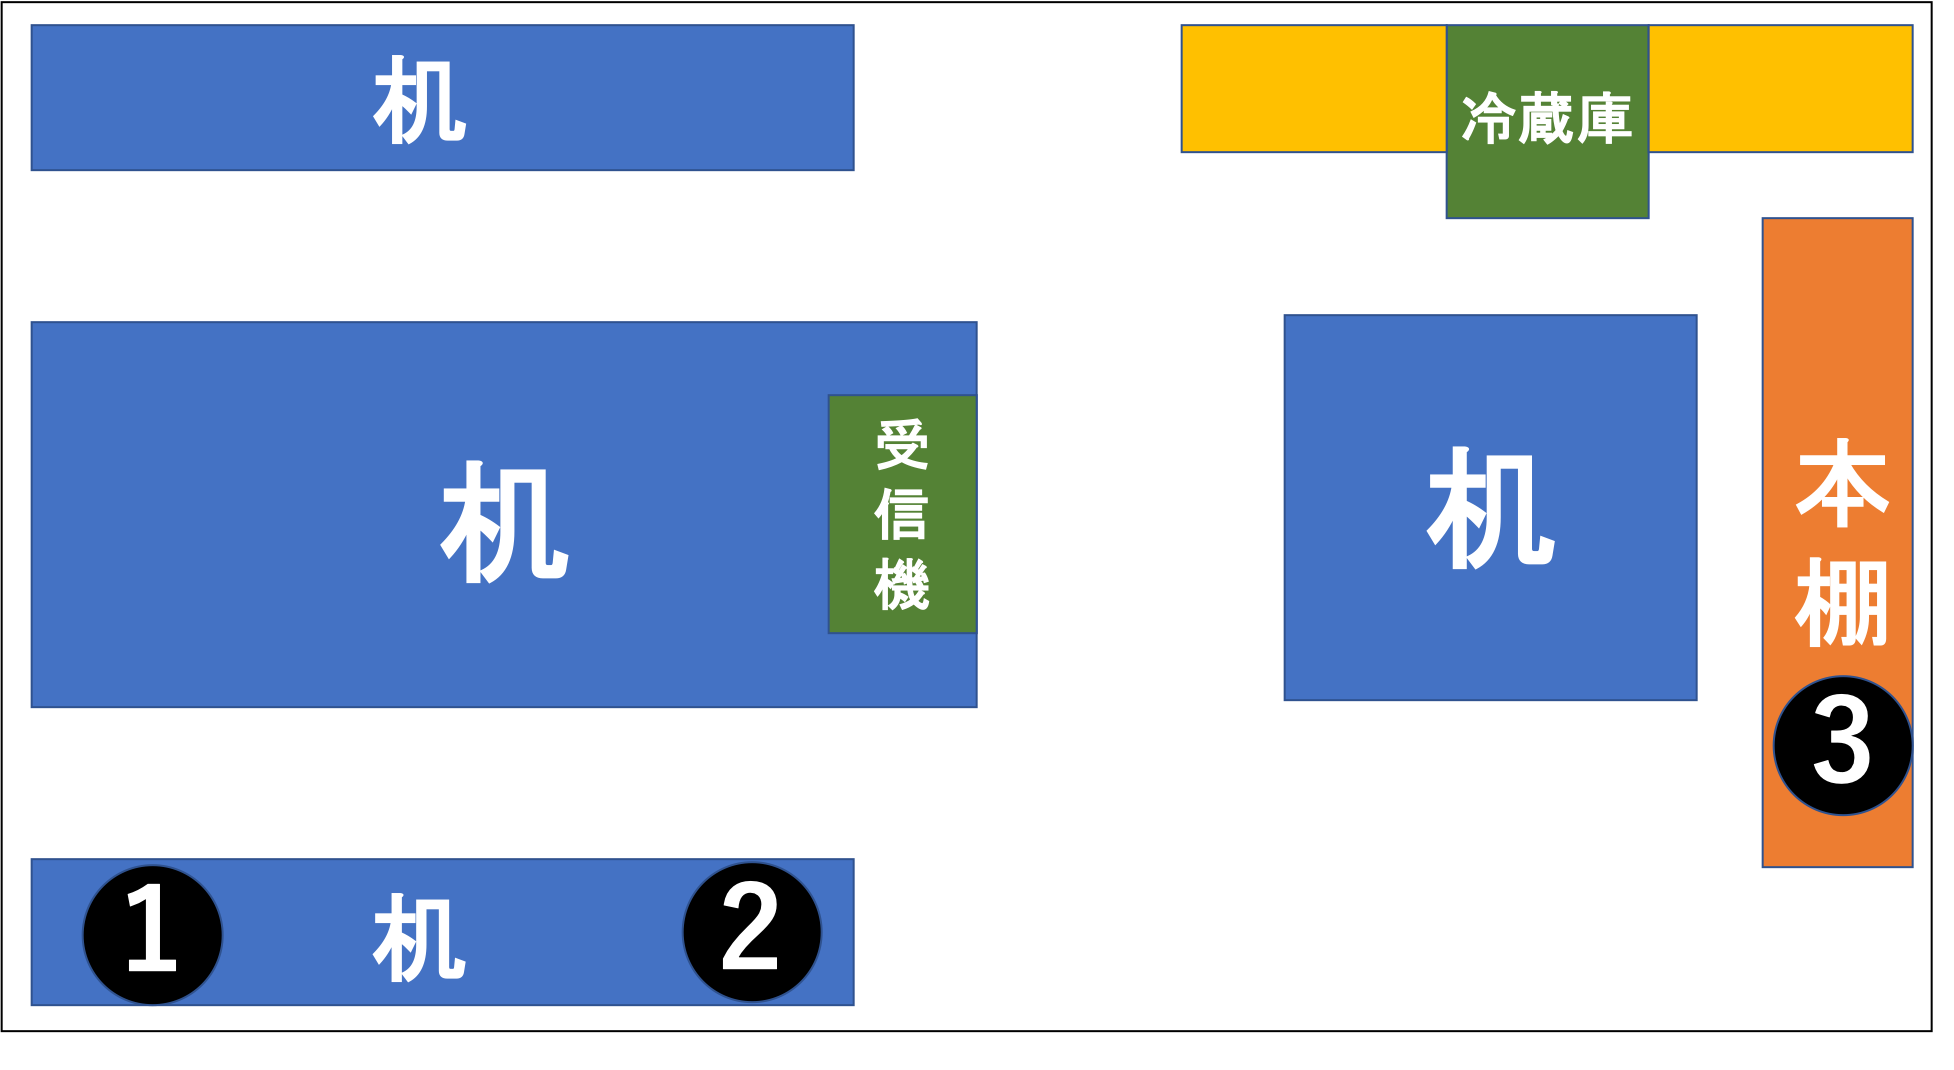
\includegraphics[width=8cm]{kinko_position_fig.png}
    \caption{金庫と受信機の位置関係図}
    \label{kinko_position}
\end{figure}

\begin{figure}[ht]
    \centering
    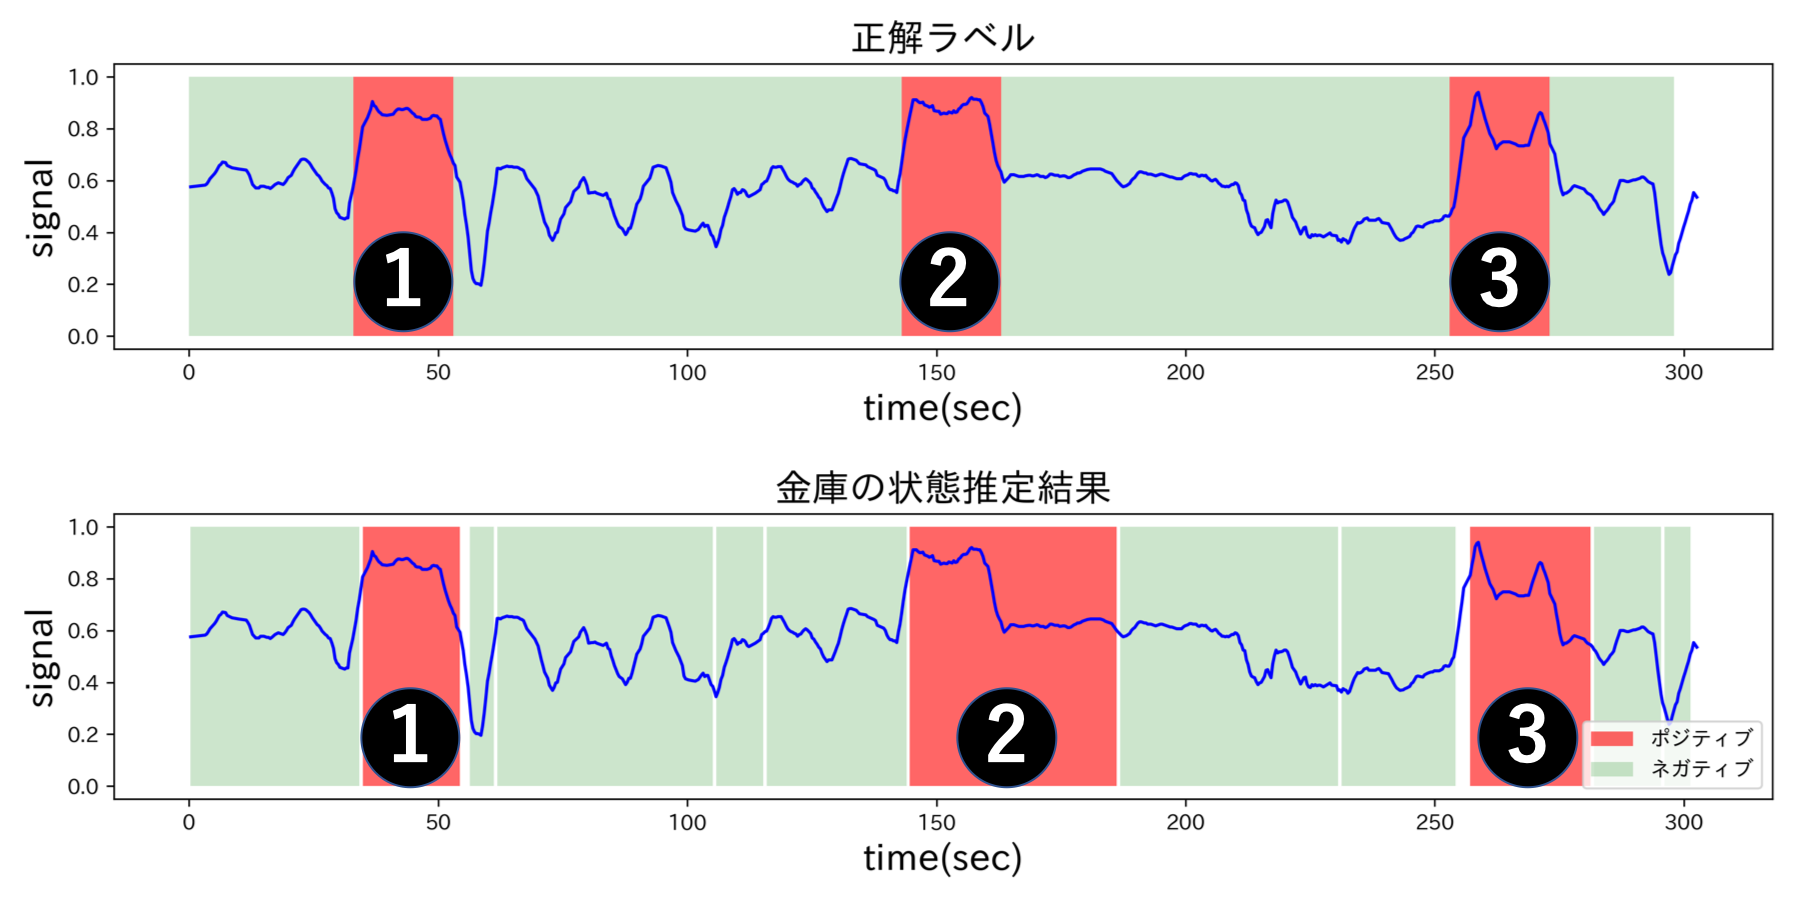
\includegraphics[width=8cm]{kinko_graph.png}
    \caption{金庫の状態推定結果グラフ}
    \label{kinko_graph}
\end{figure}

\begin{table}[htb]
    \begin{center}
        \caption{金庫の開閉における状態推定精度}
        \label{kinko_fig}
        \begin{tabular}{|c|c|c|c|} \hline
        試行回数 & 正答率 & 正解数 & 不正解数 \\ \hline
        1 & 100% & 7 & 0 \\ \hline
        2 & 100% & 7 & 0 \\ \hline
        2 & 100% & 7 & 0 \\ \hline \hline
        累計正解率 & \multicolumn{3}{c|}{100%} \\ \hline
        \end{tabular}
    \end{center}
\end{table}

\subsection{座椅子の着座における推定精度の測定}

図\ref{chair}, 図\ref{zaisu_position}のようにセンサと受信機を設置して評価実験を行った.
推定結果を図\ref{czaisu_graph}に, 正解率の一覧を表\ref{chair_fig}に示す.
図\ref{chair_graph}の白色の範囲は安定センシング区間ではない状態を 緑色の範囲はネガティブな状態(人が座っている状態)を 赤色の範囲はポジティブな状態(人が座っていない状態)を示している.
また, 図中の番号は図\ref{zaisu_position}内の番号と対応している.

同様の行動を3回行った結果, 3回とも完璧な精度で状態推定を行う事ができた.
これは座椅子は金庫や冷蔵庫と違い電波の飛ぶ方向が変わらず, また状態変化のスパンが長く安定センシング区間の判定が理想に近い環境で行われたからだと考えられる.

\begin{figure}[ht]
    \centering
    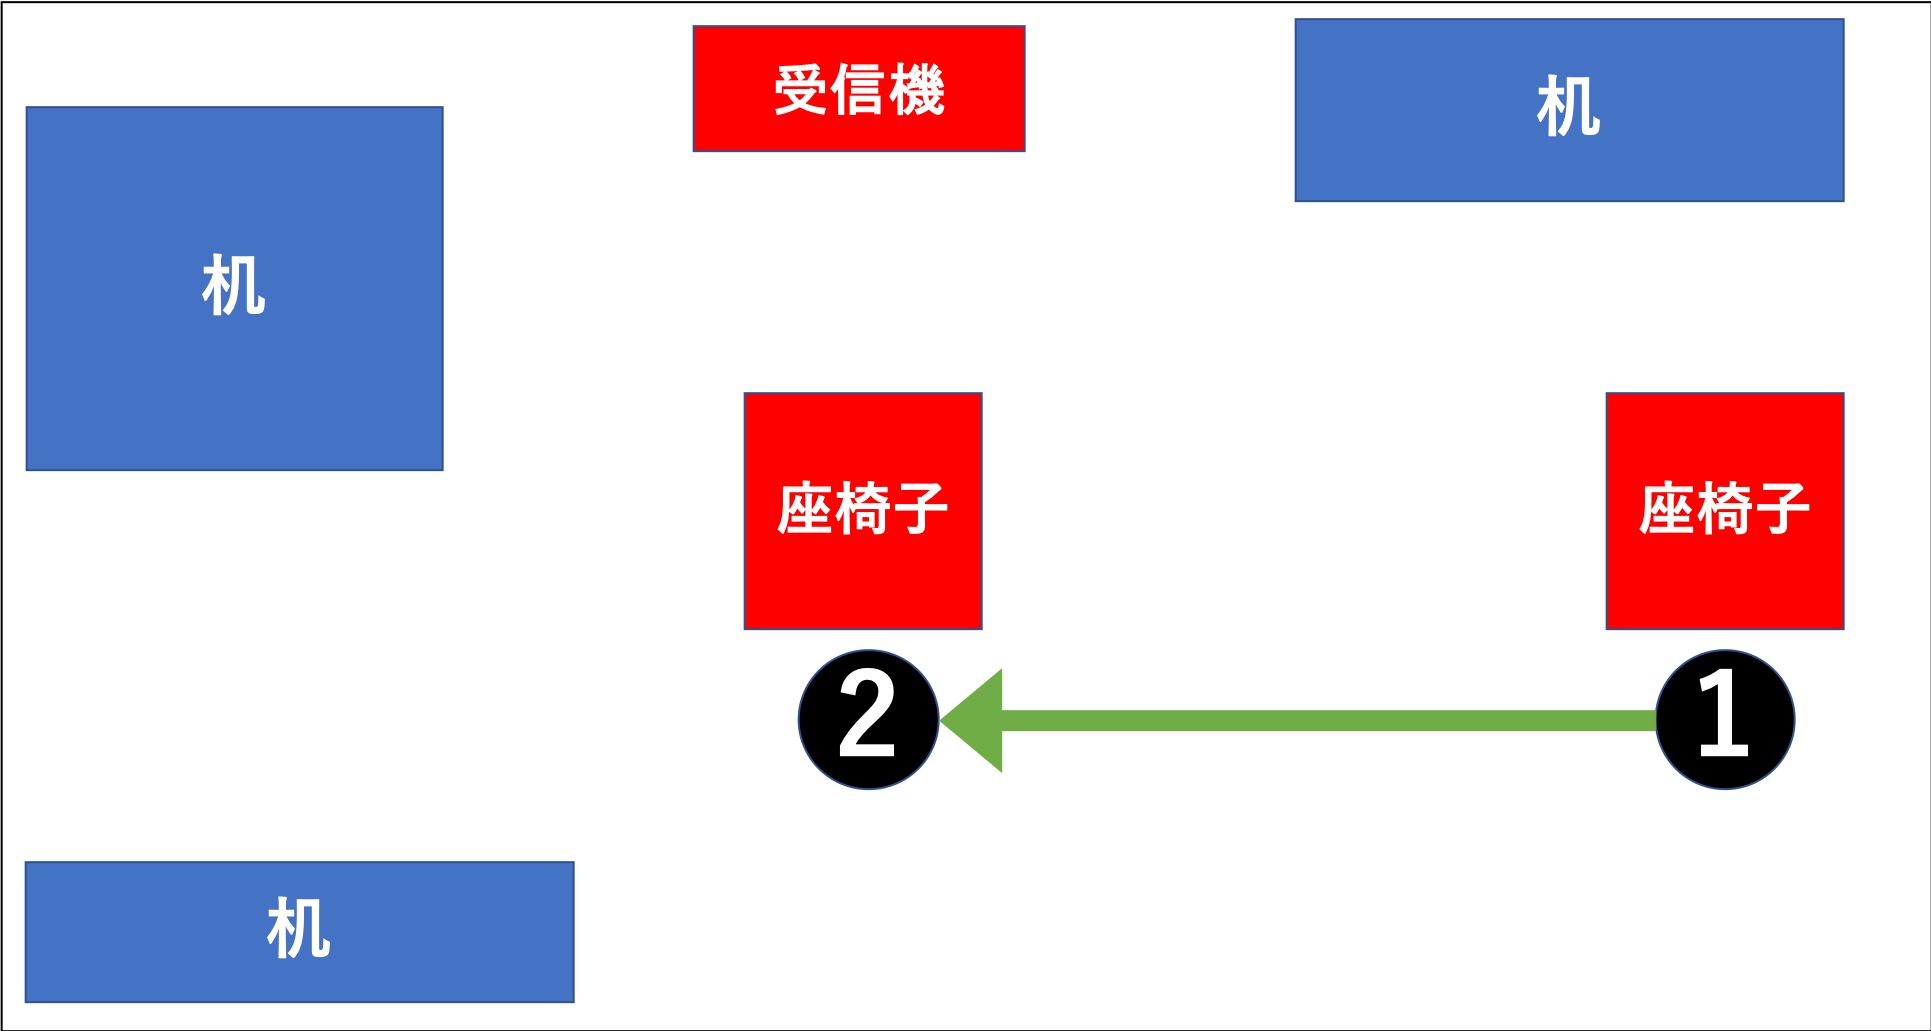
\includegraphics[width=8cm]{zaisu_position.png}
    \caption{座椅子と受信機の位置関係図}
    \label{zaisu_position}
\end{figure}

\begin{figure}[ht]
    \centering
    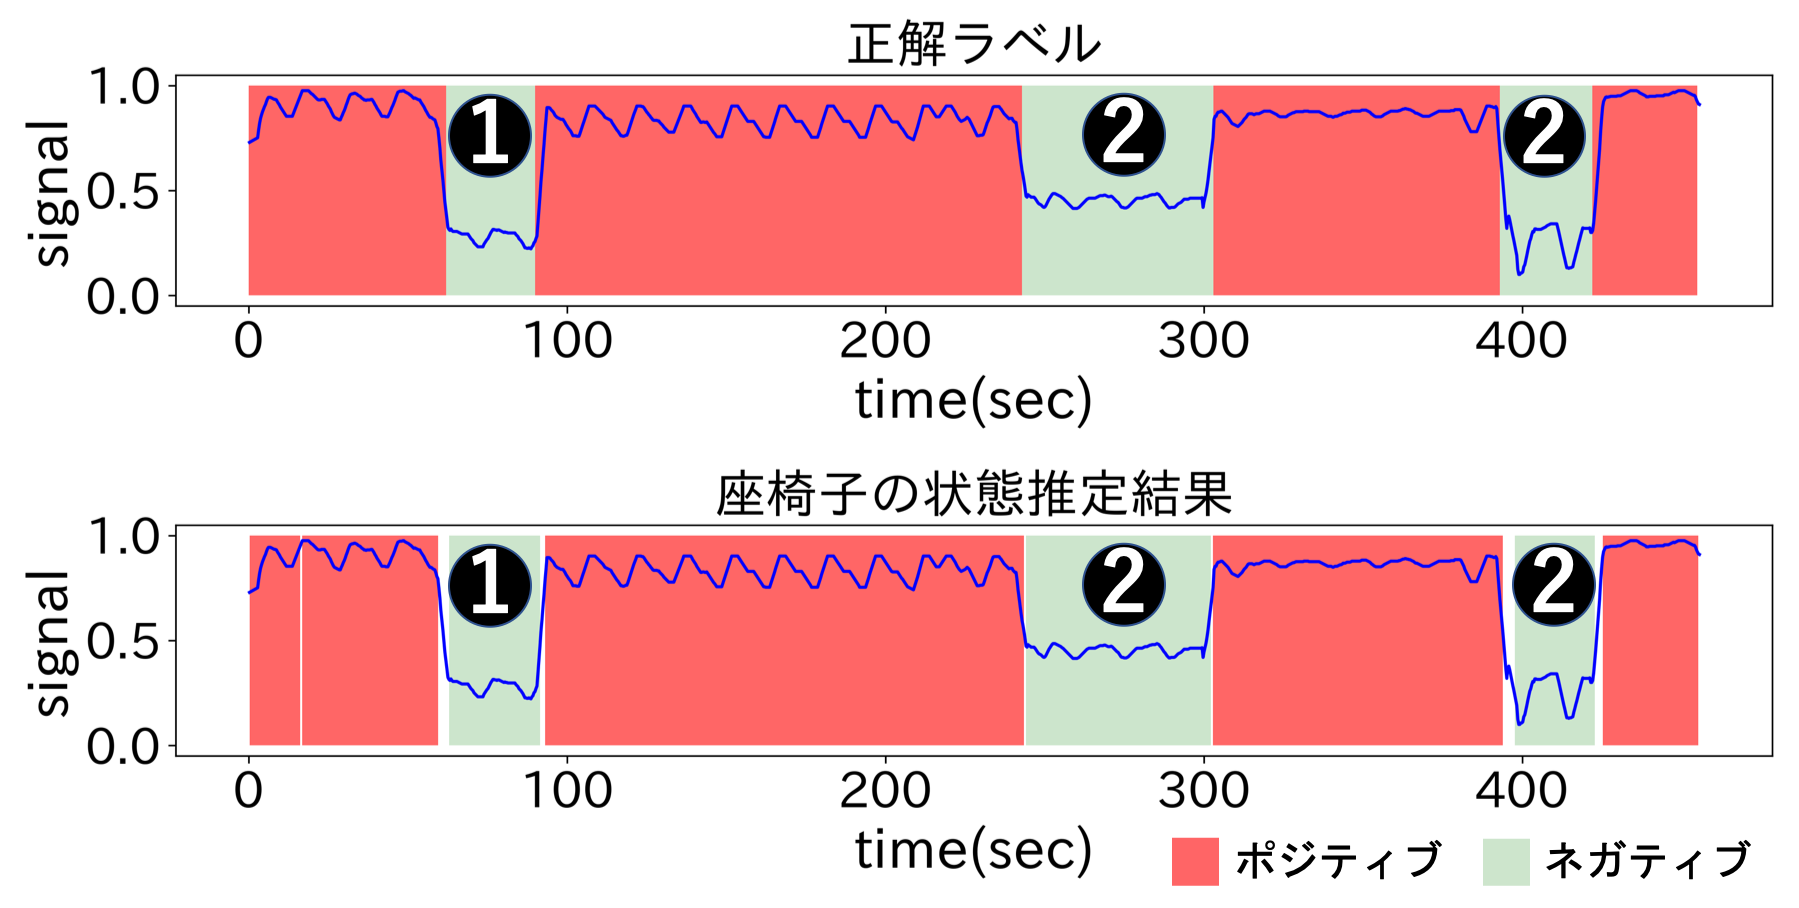
\includegraphics[width=8cm]{zaisu_graph.png}
    \caption{座椅子の状態推定結果グラフ}
    \label{chair_graph}
\end{figure}

\begin{table}[htb]
    \begin{center}
        \caption{座椅子への着席における状態推定精度}
        \label{chair_fig}
        \begin{tabular}{|c|c|c|c|} \hline
        試行回数 & 正答率 & 正解数 & 不正解数 \\ \hline
        1 & 100% & 7 & 0 \\ \hline
        2 & 100% & 7 & 0 \\ \hline
        2 & 100% & 7 & 0 \\ \hline \hline
        累計正解率 & \multicolumn{3}{c|}{100%} \\ \hline
        \end{tabular}
    \end{center}
\end{table}



%ーーーーーーーーーーーーーーーーーーーーーーーーーーーーーーーーーーーーーーーーーーーーーーーーー
%ーーーーーーーーーーーーーーーーーーーーーーーーーーーーーーーーーーーーーーーーーーーーーーーーー

\section{まとめ}
本稿ではBLEビーコンの電波強度を用いて日常の生活空間内の金庫や座椅子などのモノの状態推定を行う手法を提案した.
これまでモノの状態推定には消費電力の監視やWi-Fiの電波などが用いられてきたが, それらの手法は電気の通っていないモノや小型で移動が頻繁に行われるようなモノの状態推定には不向きであった.
そのため我々はBLEビーコンを冷蔵庫や金庫といった物体内部に設置することで, 状態変化によって変化するBLEビーコンの電波強度の変化に着目し状態推定を行うこととした.

推定を行う際, 瞬間的な変化や人などの障害物の通過などにより電波の揺らぎが発生し推定結果に影響を及ぼすことが考えられるが, 安定センシング区間という概念を利用することにより高い精度で状態推定できることを確認した.
安定センシング区間の判定にはεチューブを取り入れることで, 距離により電波強度が増幅・減衰する移動を考慮した推定を行えるようにした.
また, BLEビーコンに指向性を持たせるアダプタを取り付けることにより電波強度変化の特徴を大きく変化させ, 電波を通しやすい材質のモノであっても推定が行えるようにした.

評価実験では冷蔵庫や金庫, 座椅子にBLEビーコンを設置し日常での使用を模倣した開閉や着座動作を行い, 推定精度を確かめた.
金庫や座椅子では移動を伴っても, 共に高い精度で推定を行うことができた.
しかし電波強度の変化の具合により推定が不完全である部分もあるため, 安定センシング区間の判定や状態判定のための閾値を見直すことで改善を図っていく.

今後の課題として, 現状では安定センシング区間の判定に用いるパラメータは手動で設定しなければならず, 適切な値を探すためにあらかじめ何度か試行させる必要がある.
よってアルゴリズムを改良して自動で適切なパラメータを設定する手法の確立を目指す.


%ーーーーーーーーーーーーーーーーーーーーーーーーーーー
%ーーーーーーーーーーーーーーーーーーーーーーーーーーーーーーーーーーーーーーーーーーーーーーーーー



\begin{thebibliography}{20}
    \bibitem{soumusyo}『平成29年版情報通信白書』: 入手先 〈\url{http://www.soumu.go.jp/johotsusintokei/whitepaper/ja/h29/pdf/n3300000.pdf}〉, p.125, (参照 2019 年 4 月 24 日).
    \bibitem{TagAndThink}前川拓也, 柳沢豊, 岡留剛. Tag and Think:センサネットワークを前提としたモノ自身とその状態の推定, 情報処理学会研究報告ユビキタスコンピューティングシステム(UBI), 2007(14(2007-UBI-013)), pp. 211-218, 2007.
    \bibitem{sairyu}上田泰嵩, 梶克彦, 河口信夫. 細粒度電力センシングによる浪費電力の検出, マルチメディア、分散、協調とモバイル(DICOMO)シンポジウム論文集, pp. 1817-1821, 2010.
    \bibitem{energy}山田祐輔, 加藤丈和, 松山隆司. スマートタップネットワークを用いた家電の電力消費パターン解析に基づく人物行動推定, 研究報告ユビキタスコンピューティングシステム(UBI), 2011(4(2011-UBI-31)), pp. 1-6, 2011.
    \bibitem{redLine}江田政聡, 賀新剛, 中根傑, 横山昌平, 福田直樹, 峰野博史, 石川博, 赤外線センサを用いた在席推定に基づく照明制御手法の提案, 第4回データ工学と情報マネジメントに関するフォーラム(DEIM フォーラム 2012).
    \bibitem{WifiChannel}尾原和也, 前川卓也, 村上友規, アベセカラヒランタ. Wi-Fiチャネル状態情報を用いた教師無し学習によるドアの開閉検知手法, 情報処理学会研究報告ヒューマンコンピュータインタラクション(HCI), 2018(1(2018-HCI-180)), pp. 1-7, 2018.
    \bibitem{bleUse}LINE公式ブログ: 入手先 〈\url{http://official-blog.line.me/ja/archives/73098915.html}〉 (参照 2019 年 4 月 24 日).
    \bibitem{IoMT}堀川三好, 工藤大希, 岡本東, 村田嘉利. 移動するモノを対象とした Internet of Things の提案, 第80回全国大会講演論文集, 2018(1), pp. 471-472, 2018.
    \bibitem{tandem}浦野健太, 廣井慧, 梶克彦, 河口信夫. 配布型BLEタグとタンデムスキャナを用いた屋内位置推定手法, 情報処理学会論文誌, 60(1), pp. 58-75, 2019.
    \bibitem{blespot}渡邉洸, 高橋雄太, 大坪敦, 藤本まなと, 荒川豊, 安本慶一. BLEビーコンと反響音センシングによる屋内スポット推定, マルチメディア、 分散協調とモバイルシンポジウム2018論文集, 2018, pp. 620-626, 2018.
    \bibitem{LANgate}梶 克彦, 河口 信夫.無線 LAN 環境特異点に基づくゲート通過検出手法.
    \bibitem{en-door}Hsi-Yuan Tsai, Guan-Heng Chen, Huang-Chen Lee. Using low-cost, non-sensor-equipped BLE beacons to track people's movements, IPSN '17 Proceedings of the 16th ACM/IEEE International Conference on Information Processing in Sensor Networks, pp. 291-292, 2017.
    \bibitem{BLEpkpk}池田翔太, 梶克彦. BLEビーコンをパカパカ, マルチメディア、分散協調とモバイルシンポジウム2016論文集, 2016, pp. 899-904, 2016.
    \bibitem{sensing-area}梶克彦, 河口信夫. 安定センシング区間検出に基づく3次元歩行軌跡推定手法, 情報処理学会論文誌, Vol.57, No.1, pp.12-24, 2016.
    \bibitem{ips-chube}吉澤実, 高崎航, 大村廉. 加速度ベース行動認識におけるレスポンス時間短縮のためのパラメータ検討, 情報処理学会マルチメディア,分散協調とモバイル(DICOMO2013)シンポジウム論文集, pp. 647-654, 2013.
    %\bibitem{en-AreaUsed}Rachael Purta, Aaron Striegel. Estimating dining hall usage using bluetooth low energy beacons, UbiComp '17 Proceedings of the 2017 ACM International Joint Conference on Pervasive and Ubiquitous Computing and Proceedings of the 2017 ACM International Symposium on Wearable Computers, pp. 518-523, 2017.
\end{thebibliography}


\end{document}